\documentclass{beamer}
% This is the file main.tex
\usetheme{Dresden}
\usepackage{tikz}
\setbeamertemplate{navigation symbols}{}
\setbeamertemplate{mini frames}{}
\renewcommand*{\slideentry}[6]{}
\addtobeamertemplate{navigation symbols}{}{%
    \usebeamerfont{footline}%
    \usebeamercolor[fg]{footline}%
    \hspace{1em}%
    \insertframenumber/\inserttotalframenumber
}
\setbeamercolor{structure}{fg=MyPurple}
\definecolor{MyPurple}{RGB}{105,18,83}
\usepackage{graphicx}
\usepackage{amsmath}
\usepackage[euler]{textgreek}
\usepackage{adjustbox}
\usepackage{booktabs}
\usepackage{multirow}
\usepackage{multirow, xspace, amsmath}
\usepackage{pdfpages}
\usepackage{fancybox}
\usepackage{stackengine}
\usepackage{cancel}
%\usepackage{geometry}
%\geometry{
% a4paper,
% total={170mm,257mm},
% left=20mm,
% top=20mm,
% }
\newcommand*{\ttbar}{\ensuremath{t\bar{t}}\xspace}
\newcommand*{\mbb}{\ensuremath{\text{m}_{bb}}\xspace}
\newcommand*{\dsig}{\ensuremath{|\sigma_{d_{0}}|}\xspace} 
\newcommand*{\met}{\ensuremath{\cancel{E_{T}}}\xspace}
\newcommand{\backupbegin}{
   \newcounter{framenumberappendix}
   \setcounter{framenumberappendix}{\value{framenumber}}
}
\newcommand{\backupend}{
   \addtocounter{framenumberappendix}{-\value{framenumber}}
   \addtocounter{framenumber}{\value{framenumberappendix}} 
}
\newcommand\tab[1][1cm]{\hspace*{#1}}

\newcommand*{\header}[1]{\fontsize{16}{8}\selectfont \textbf{{\color{MyPurple}{#1}}}}

\usepackage{tikz}
\usepackage[compat=1.1.0]{tikz-feynman}


\title{Search For Double Higgs Production in the $b\bar{b}WW^{*}$ Channel}
\subtitle{}
\author[John C.S. Myers]{John C.S. Myers}
\institute[University of Oregon]{ University of Oregon}
\date{\today}

\begin{document}

\titlepage
%%Start with general into and then briefly on trigger
%% highlight talks and being public face
%%
%%need to think of transiton into HHbbWW
%%
%%HHbbWW paper analysis-->leptons inside jets-->how to use ANL computing


\begin{frame}
\begin{center}
\header{About Me}
\end{center}
\begin{columns}
\begin{column}{0.8\textwidth}
\begin{itemize}
\small
\item{B.Sc. at Ohio State University, 2013}
\begin{itemize}
\footnotesize
\item Worked with Harris Kagan and KK. Gan on accelerated lifetime testing for IBL optical readouts
\end{itemize}
\item Began work at UO with Stephanie Majewski in 2013
\begin{itemize}
\footnotesize
\item Worked on LAr Phase-II Upgrade TDR
\end{itemize}
\end{itemize}
\end{column}
\begin{column}{0.2\textwidth}
\begin{center}
\vspace{-1cm}
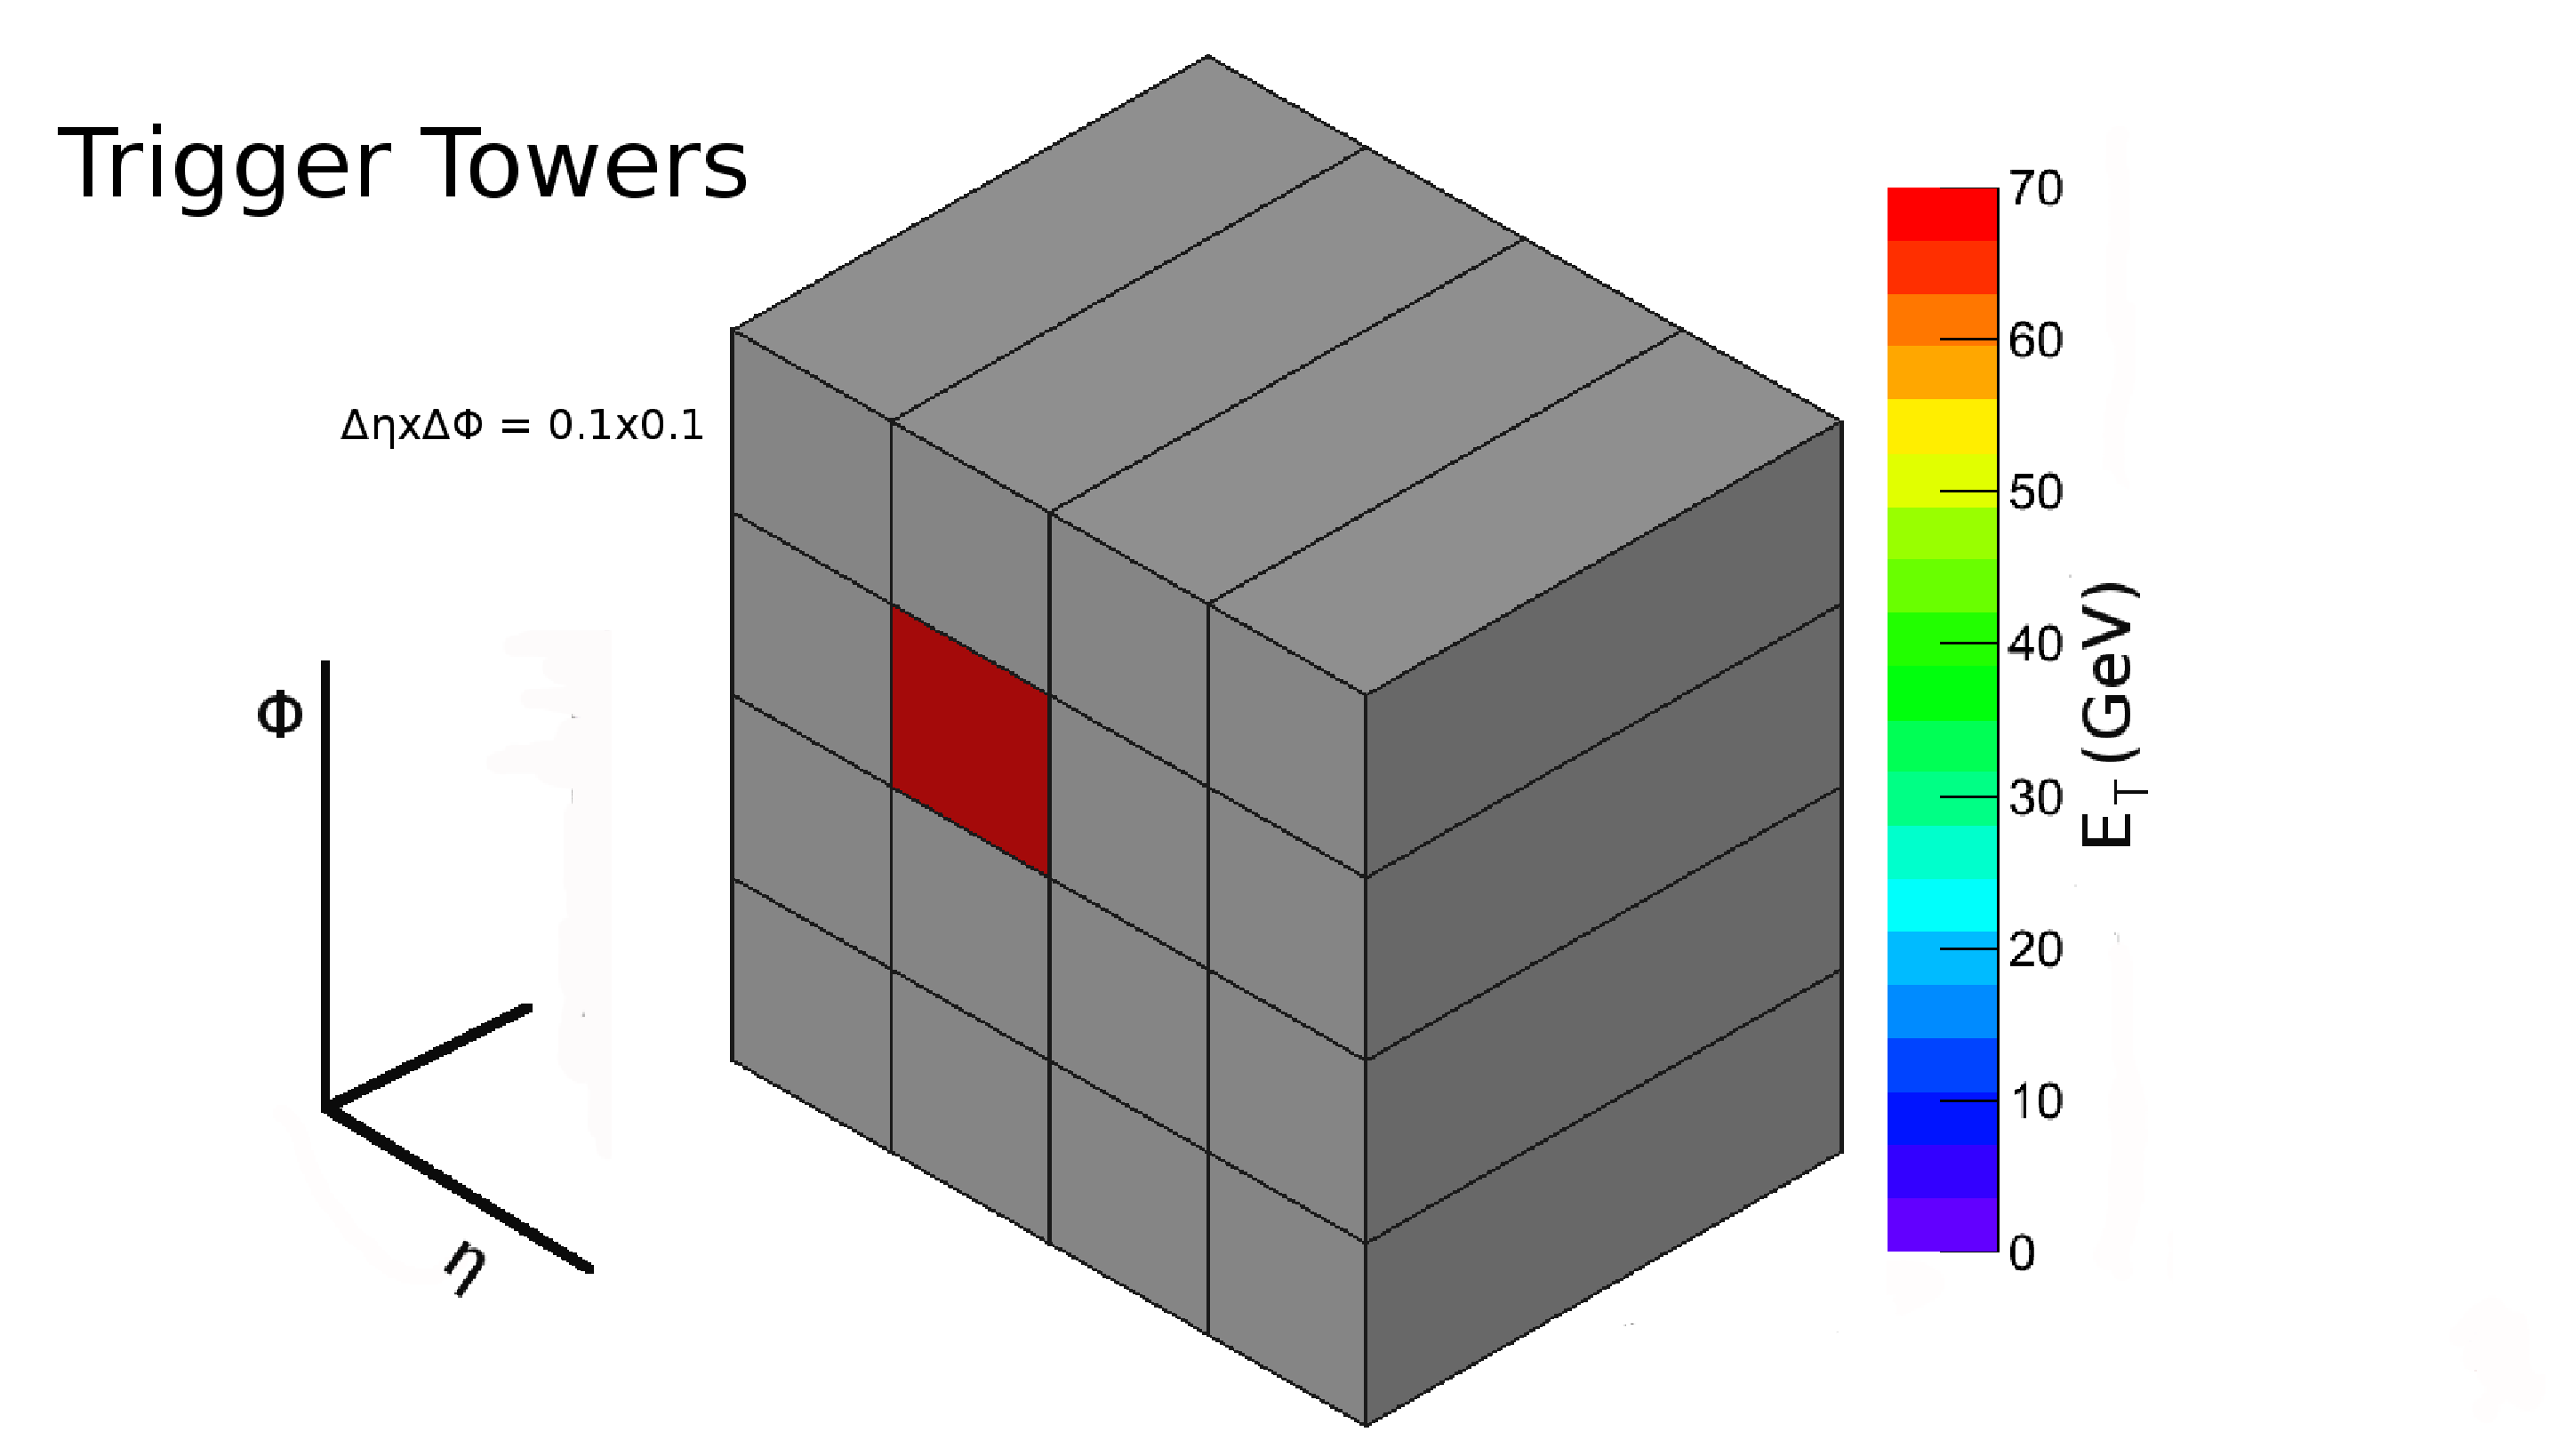
\includegraphics[width=1.2\textwidth]{figures/fig_01a}\\
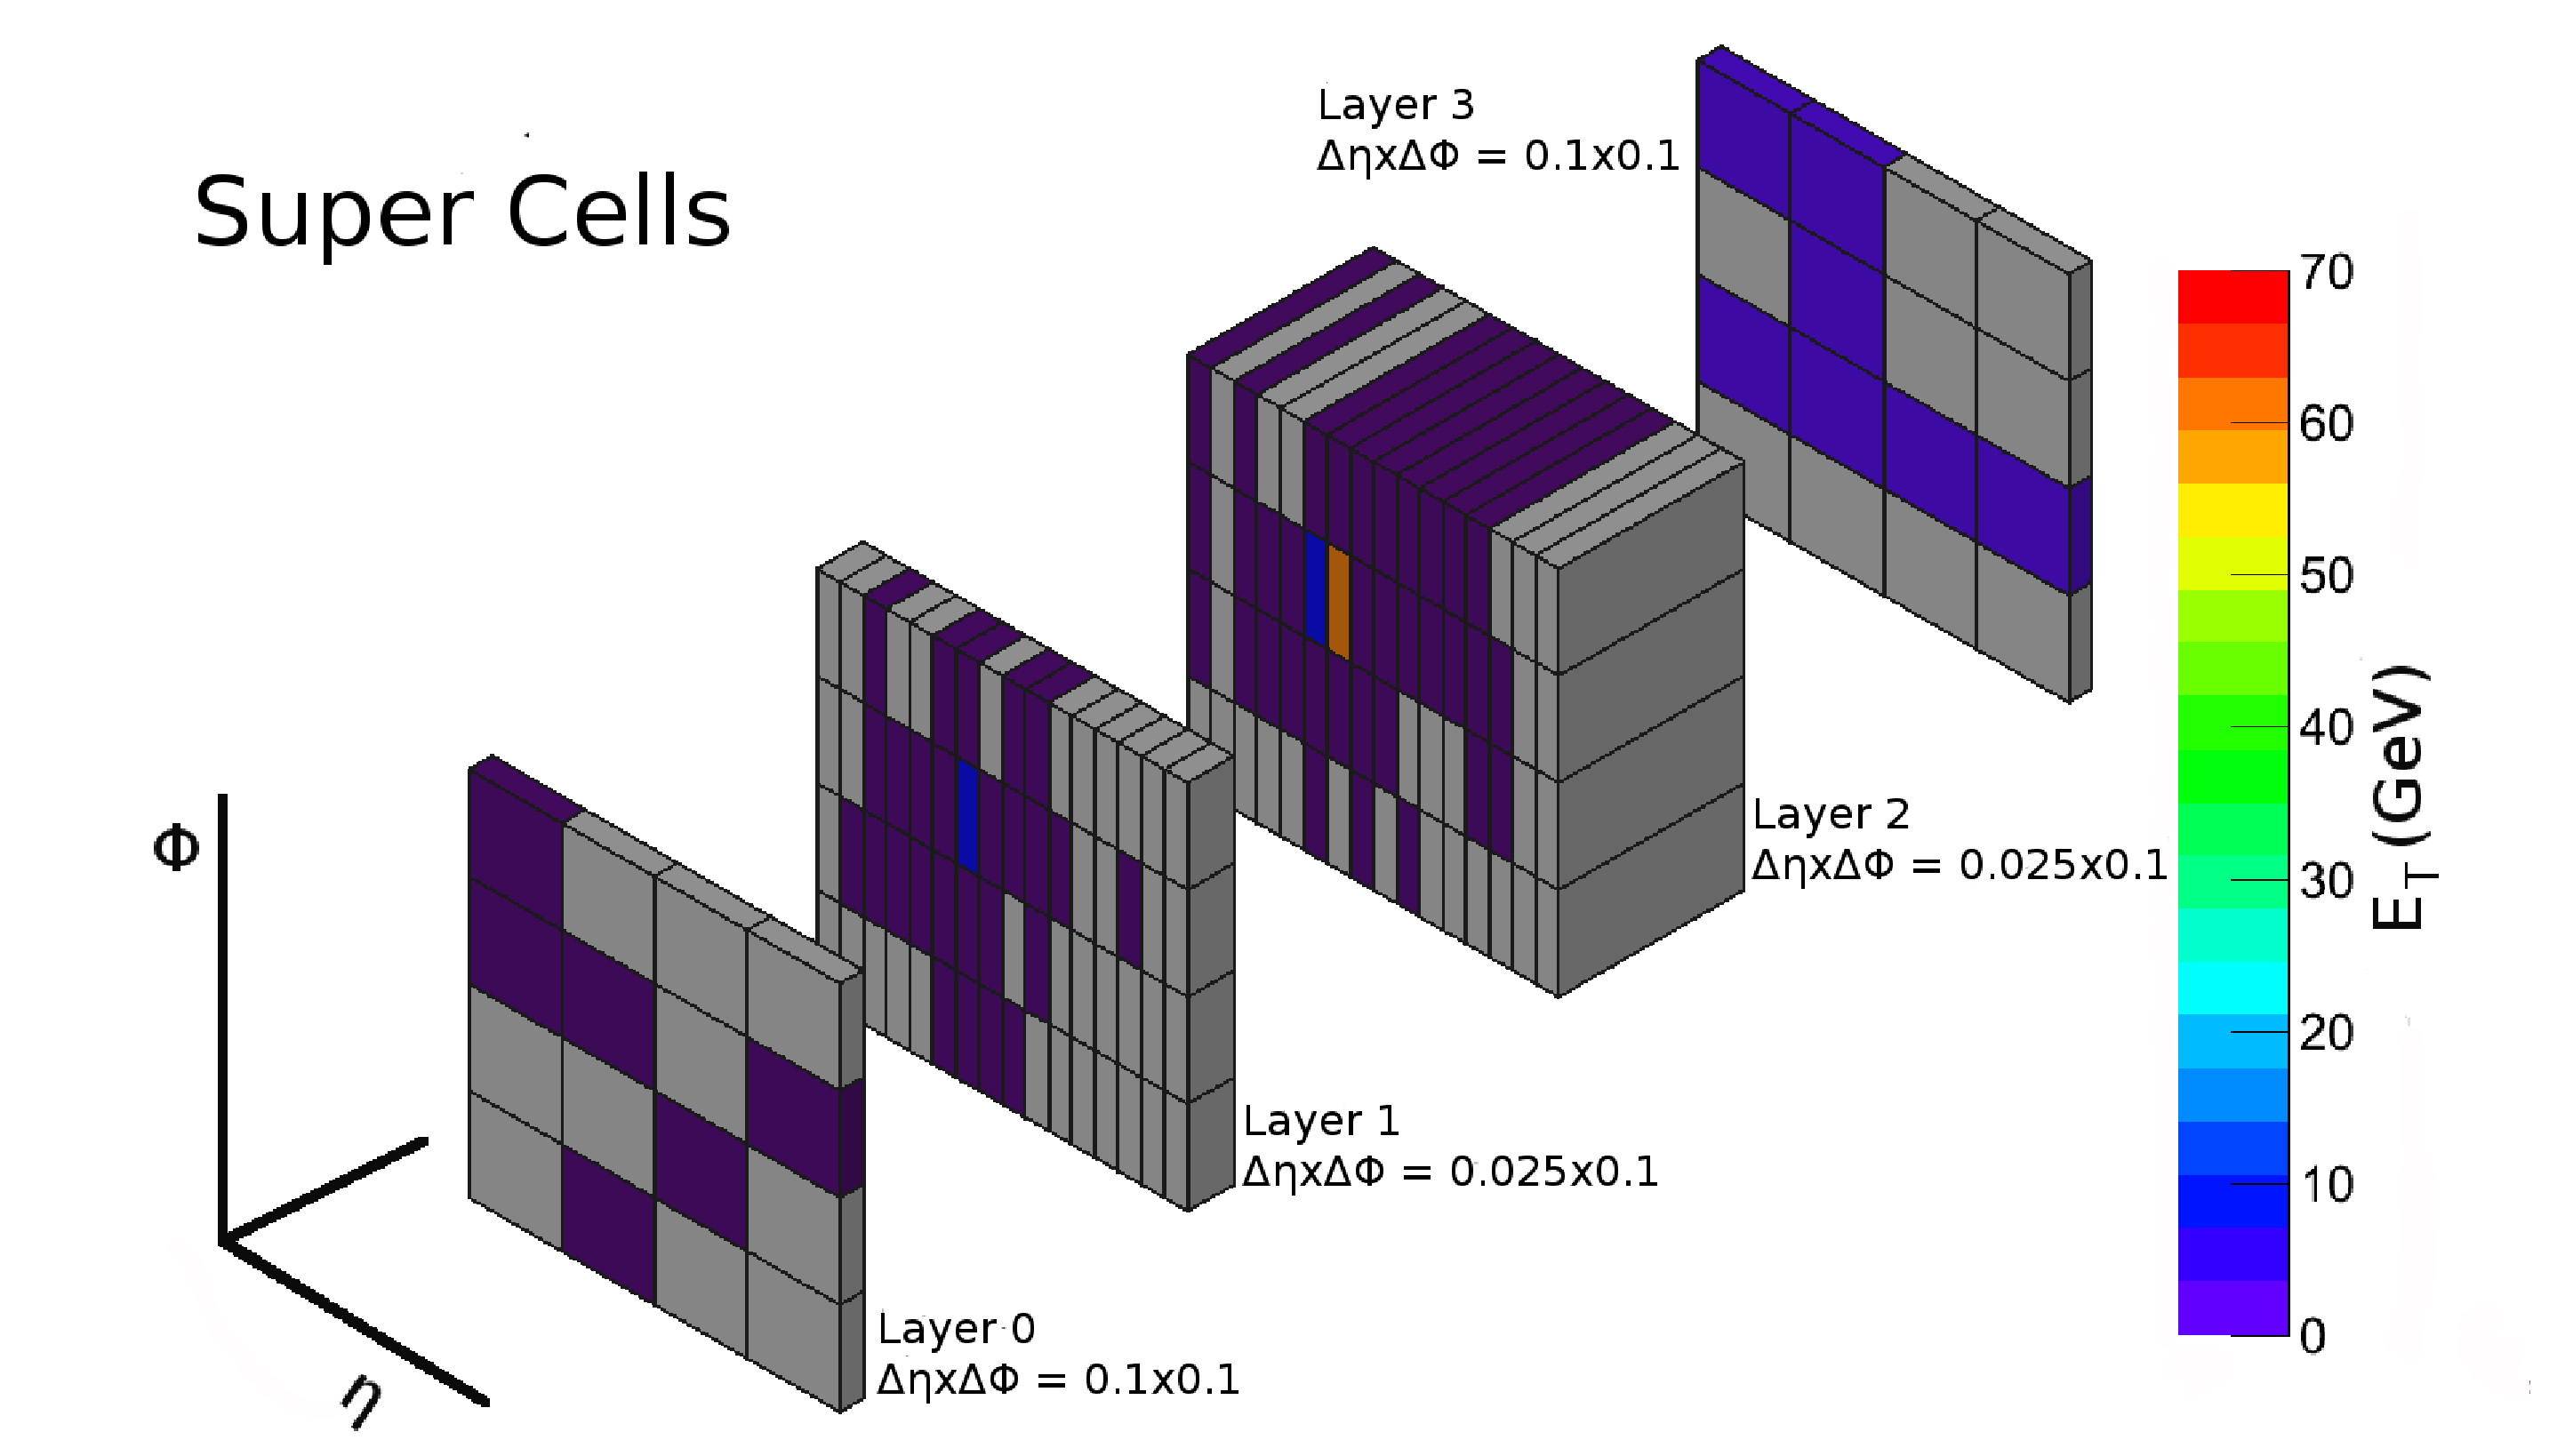
\includegraphics[width=1.2\textwidth]{figures/fig_01b}
\end{center}
\end{column}
\end{columns}
\begin{itemize}
\small
\item Began working with Eric Torrence in 2015 on $\tau$ trigger upgrade studies Qualification task
\item Started work on full Run 2 Boosted $HH\rightarrow{}b\bar{b}WW^{*}$ analysis
\begin{itemize}
\footnotesize
\item 2015-2016 analysis needed manpower to move toward publication
\end{itemize}
\item Started working as HLT Reprocessing Expert in 2017
\begin{itemize}
\item Moved to Coordinator within 9 months
\end{itemize}
\item Served as Trigger Online On-call during 2018
\end{itemize}
\end{frame}

\begin{frame}
\begin{center}
\header{Motivation}
\end{center}
\begin{columns}
\begin{column}{0.5\textwidth}
\textcolor{MyPurple}{SM di-Higgs production}\\
\begin{itemize}
\item Two dominant production modes
\item Destructively interfere 
\item Gives very small cross section 
\item Measurement of trilinear Higgs coupling is an important measurement for the HL-LHC
\end{itemize}
\end{column}
\begin{column}{0.5\textwidth}
\begin{figure}[h]
\footnotesize
\begin{center}
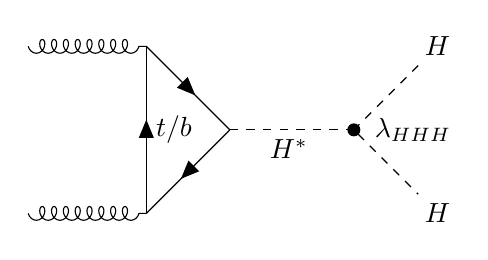
\begin{tikzpicture}
\begin{feynman}
\vertex (i1);
\vertex [right = of i1] (t1);
\vertex [dot][below right =of t1] (t3);
\vertex [below left= of t3] (t2);
\vertex [left = of t2] (i2);
\vertex [right =of t3][dot](h){};
\vertex [above right = of h] (f1){\(H\)};
\vertex [below right = of h] (f2){\(H\)};
\diagram* {
(i1) -- [gluon] (t1),
(i2) -- [gluon] (t2),
(t1) -- [fermion](t3) -- [fermion] (t2) -- [fermion,edge label'=\(t/b\)](t1),
(t3) -- [scalar,edge label'=\(H^{*}\)] (h),
(f1) -- [scalar] (h) -- [scalar](f2)
};
\vertex [right=0.75cm of h] {\(\lambda_{HHH}\)};
\end{feynman}
\end{tikzpicture}
\hspace{1cm}
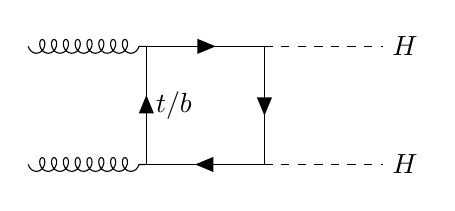
\begin{tikzpicture}
\begin{feynman}
\vertex (i1);
\vertex [ right = of i1] (t1);
\vertex [right = of t1] (t2);
\vertex [below = of t2] (t3);
\vertex [left = of t3] (t4);
\vertex [ left=of t4] (i2);
\vertex [ right =of t2] (f1){\(H\)};
\vertex [ right=of t3] (f2){\(H\)};
\diagram* {
(i1) -- [gluon] (t1),
(i2) -- [gluon] (t4),
(t1) -- [fermion](t2) -- [fermion] (t3) -- [fermion](t4) -- [fermion,edge label'=\(t/b\)] (t1),
(t2) -- [scalar] (f1),
(t3) -- [scalar] (f2)
};
\end{feynman}
\end{tikzpicture}
\end{center}
\end{figure}
\end{column}
\end{columns}
\end{frame}

\begin{frame}
\begin{center}
\header{Motivation}
\end{center}
\begin{columns}
\begin{column}{0.5\textwidth}
\textcolor{MyPurple}{Resonant di-Higgs production}\\
\begin{itemize}
\itemDuring Run 2, more interesting to perform search for BSM production
\item Eg: Heavy Higgs-like Scalar
\begin{itemize}
\item Couples to SM Higgs
\item Large enhancement to HH production rate
\end{itemize}
\item This was the original focus of my thesis
\end{itemize}
\end{column}
\begin{column}{0.5\textwidth}
\begin{figure}[h]
\footnotesize
\begin{center}
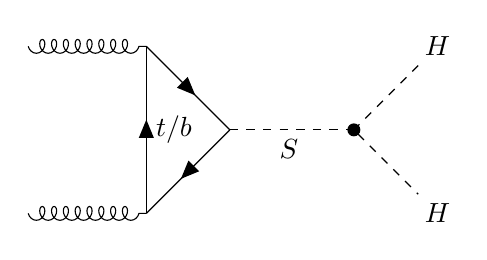
\begin{tikzpicture}
\begin{feynman}
\vertex (i1);
\vertex [right = of i1] (t1);
\vertex [dot][below right =of t1] (t3);
\vertex [below left= of t3] (t2);
\vertex [left = of t2] (i2);
\vertex [right =of t3][dot](h){};
\vertex [above right = of h] (f1){\(H\)};
\vertex [below right = of h] (f2){\(H\)};
\diagram* {
(i1) -- [gluon] (t1),
(i2) -- [gluon] (t2),
(t1) -- [fermion](t3) -- [fermion] (t2) -- [fermion,edge label'=\(t/b\)](t1),
(t3) -- [scalar,edge label'=\(S\)] (h),
(f1) -- [scalar] (h) -- [scalar](f2)
};
\end{feynman}
\end{tikzpicture}
\end{center}
\end{figure}
\end{column}
\end{columns}
\end{frame}

\begin{frame}
\begin{center}
\header{$b\bar{b}WW^{*}$ semi-leptonic channel}
\end{center}
\vspace{-0.6cm}
\begin{columns}
\begin{column}{0.4\textwidth}
\begin{itemize}
\small
\item Lower QCD background but more \ttbar than 4b 
\item Lepton is strong discriminate for QCD but decay contains neutrino
\item This search is not currently competitive for SM measurement
\item Could be competitive at large resonant mass
\end{itemize}
\end{column}
\begin{column}{0.6\textwidth}
\begin{center}
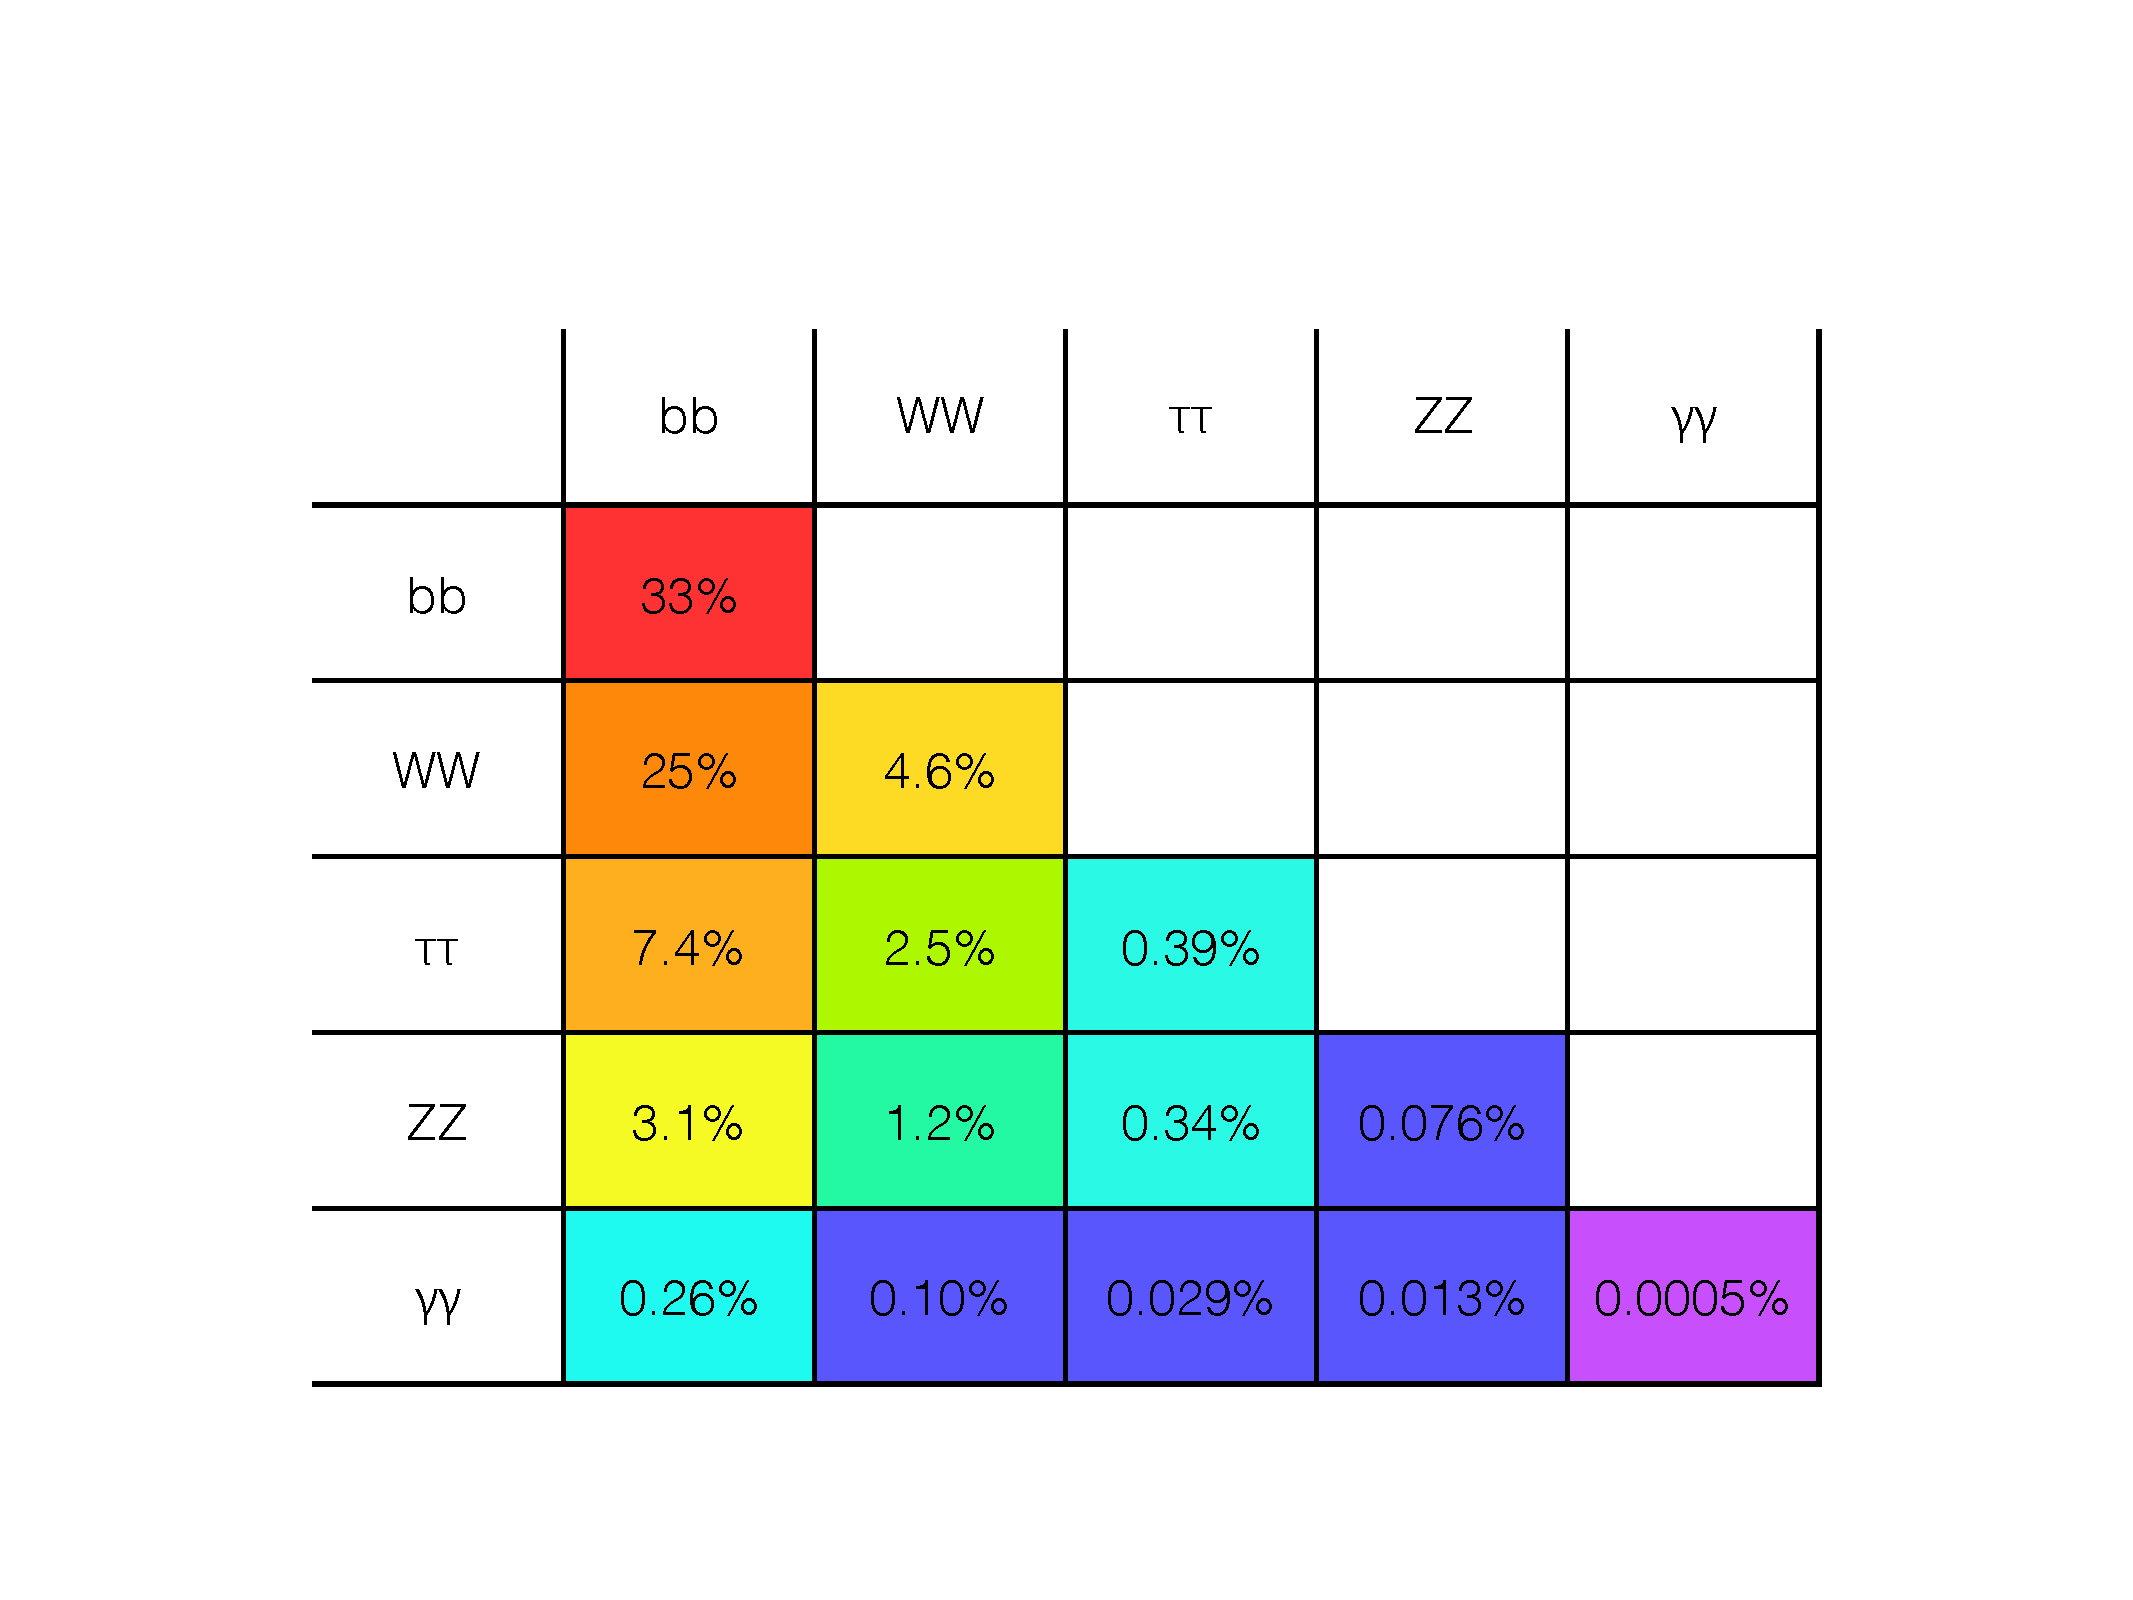
\includegraphics[width=0.75\textwidth]{figures/DiHiggsBRs}\\
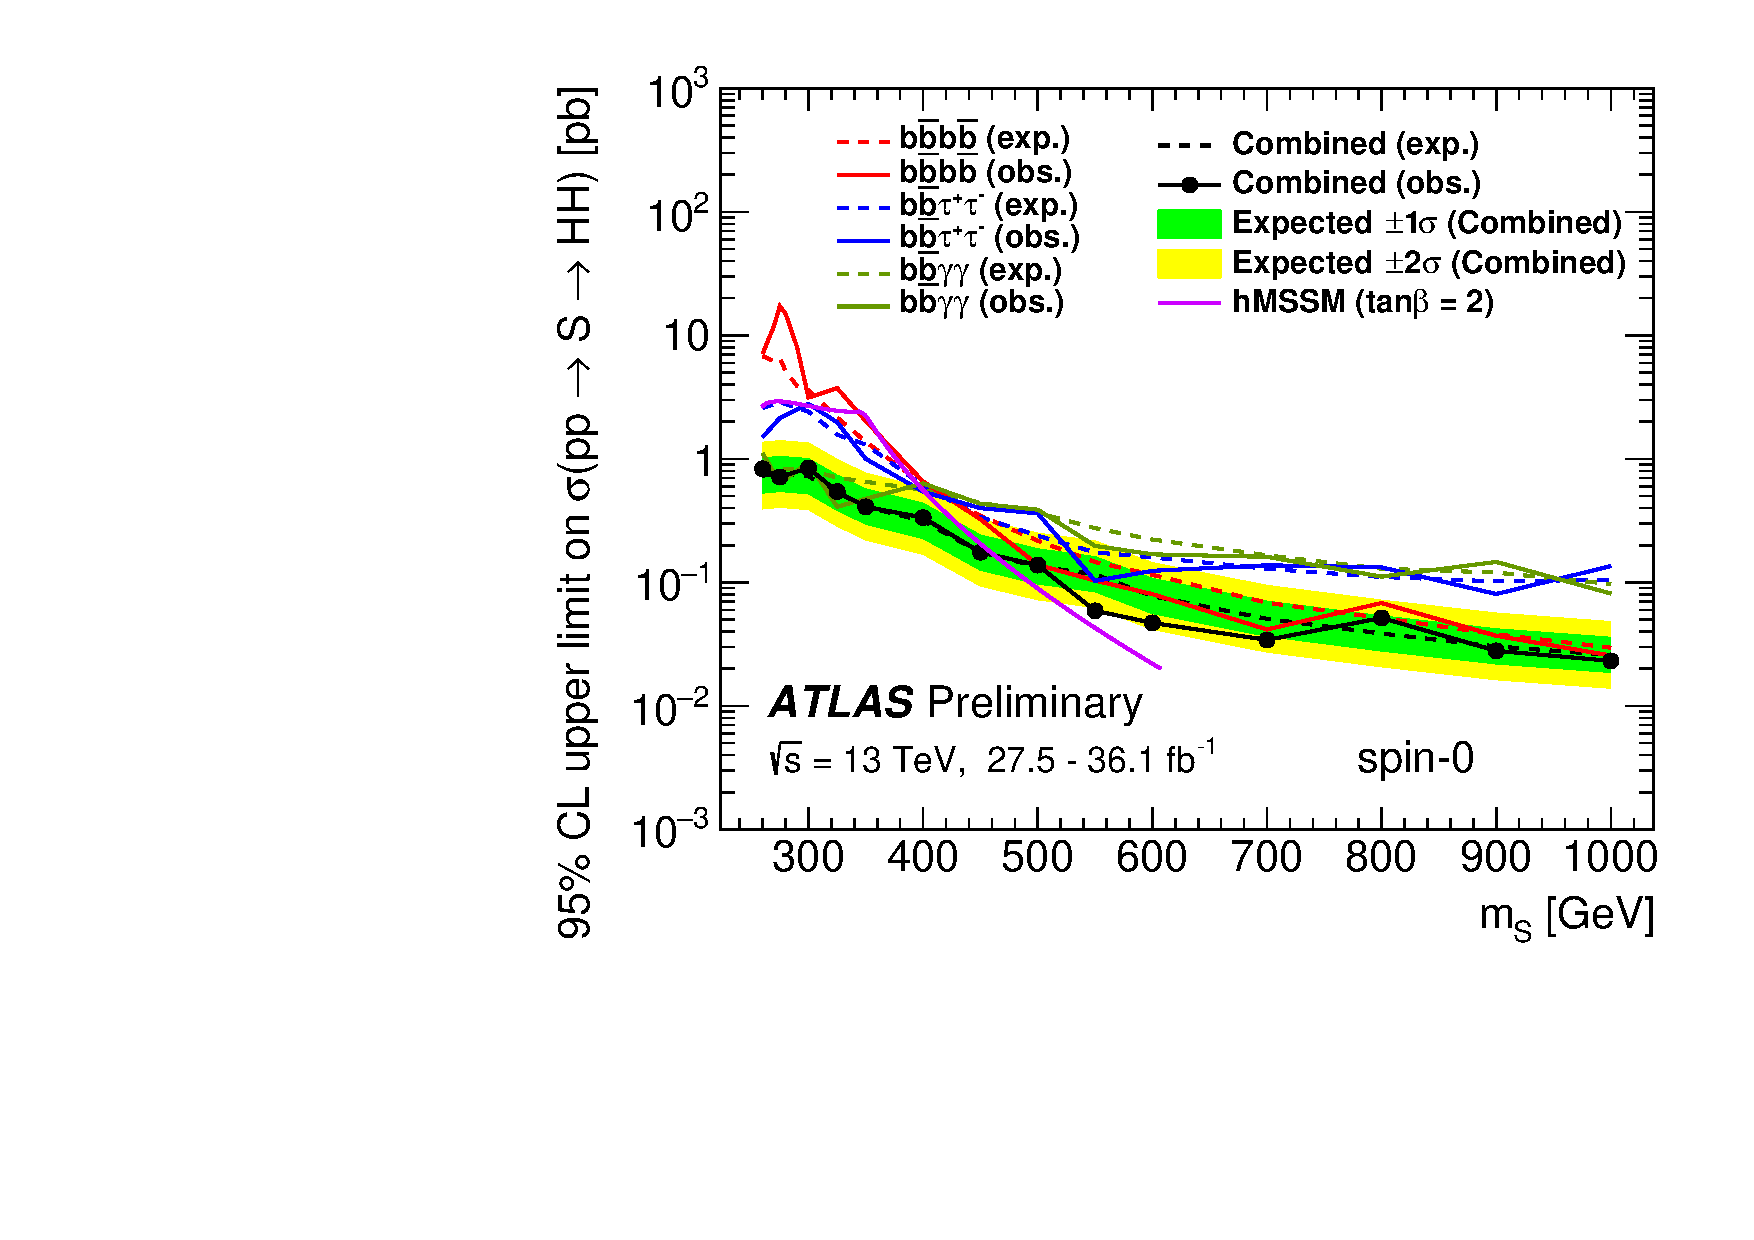
\includegraphics[width=0.75\textwidth]{figures/comb_limit}
\end{center}
\end{column}
\end{columns}
\end{frame}


\begin{frame}
\begin{center}
\header{$\mathbf{HH\rightarrow b\bar{b}WW}$ Analysis Strategy}
\end{center}
\begin{columns}
\begin{column}{0.5\textwidth}
\begin{center}
\vspace{-0.2cm}
\color{MyPurple}{Resolved Analysis}
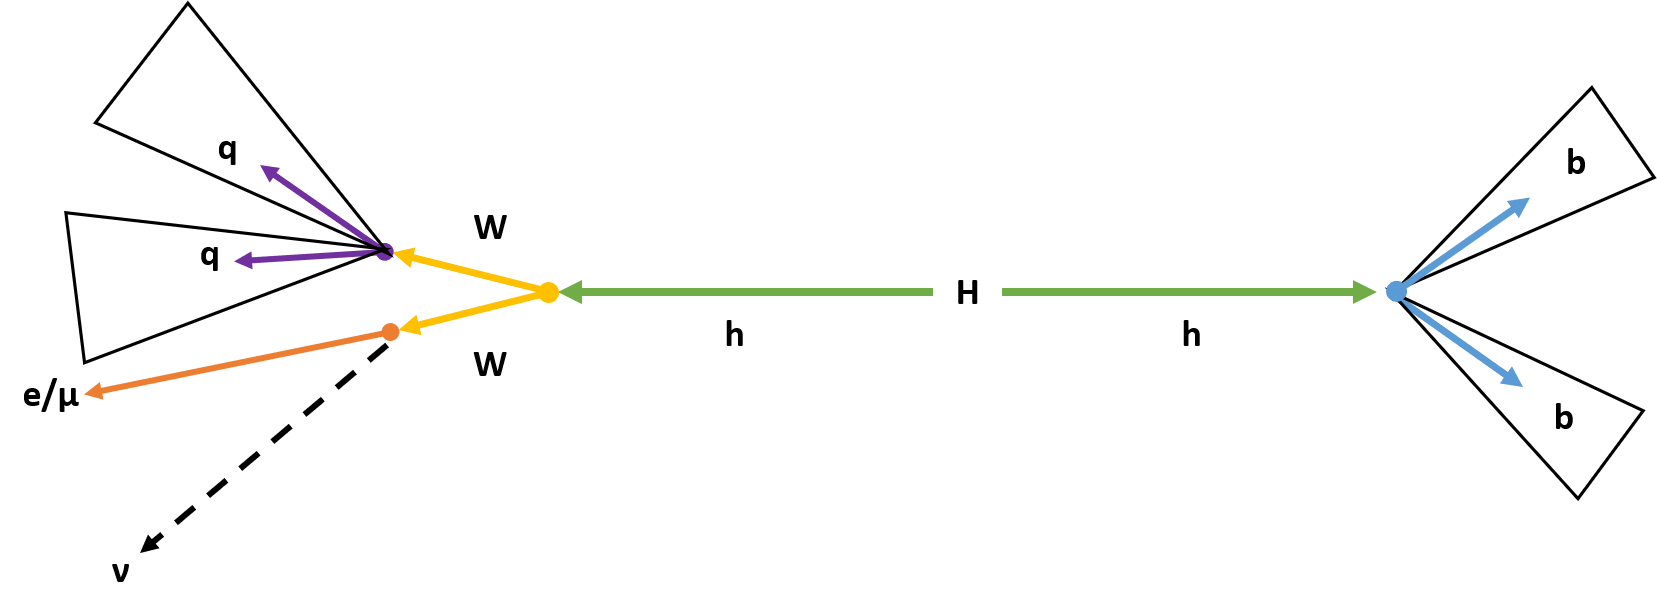
\includegraphics[width=1\textwidth]{figures/resolved_topo}
\end{center}
\begin{itemize}
\item SM production is not very boosted
\item A resolved topology is used for a SM, non-resonant measurement and a low mass resonance search
\end{itemize}
\end{column}
\begin{column}{0.5\textwidth}
%\vspace{-0.5cm}
\begin{center}
\color{MyPurple}{Boosted Analysis}
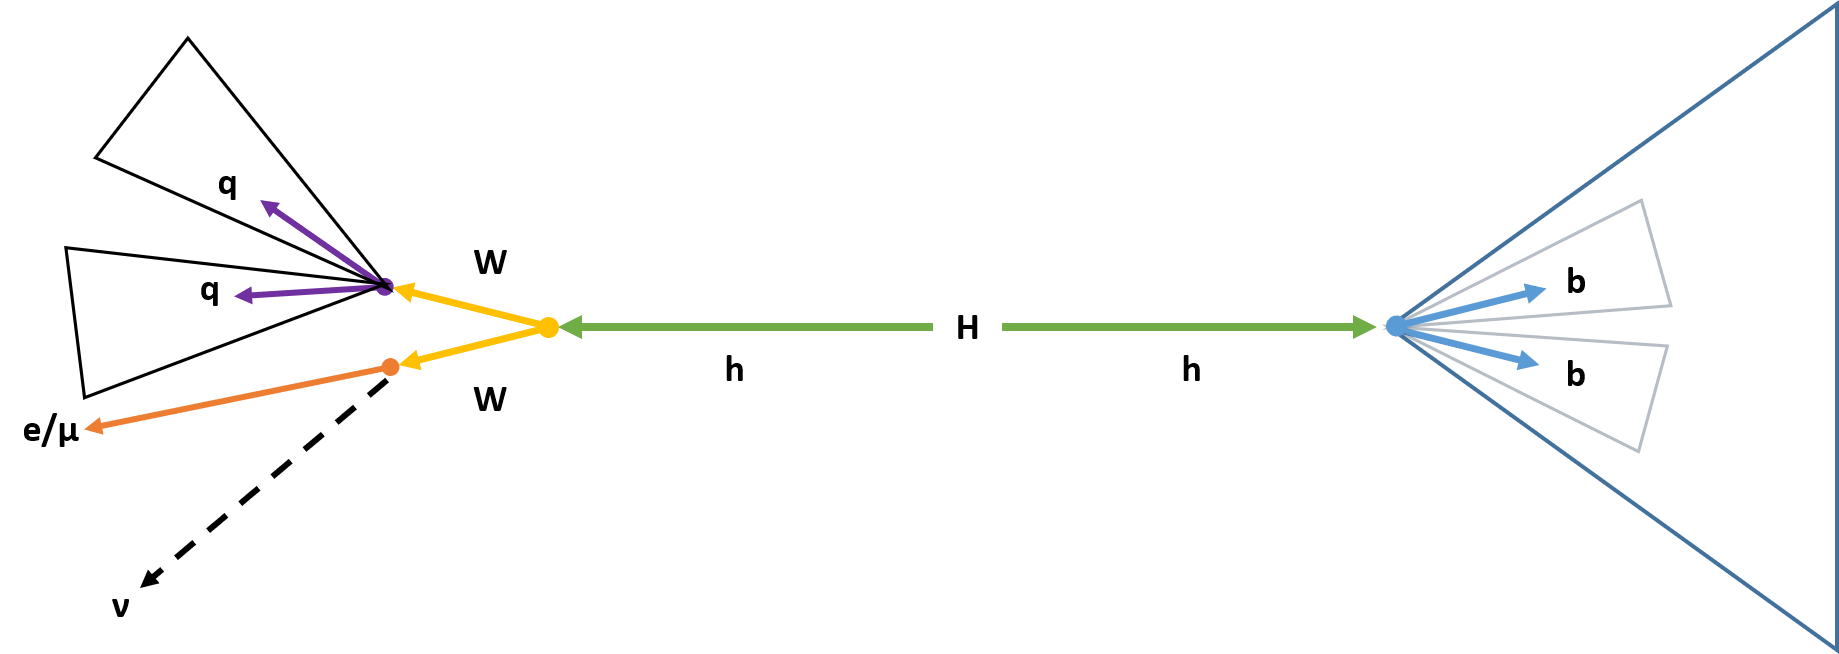
\includegraphics[width=1\textwidth]{figures/boosted_topo}
\end{center}
\begin{itemize}
\item As the resonant mass increases, the system becomes more boosted
\item Boosted analysis focuses on high resonant masses (1-3 TeV)
\end{itemize}
\end{column}
\end{columns}
\end{frame}

\begin{frame}
\begin{center}
\header{Data and Background}
\end{center}
\begin{columns}
\begin{column}{0.3\textwidth}
\small
\color{MyPurple}{Final State}
\begin{itemize}
\item $b\bar{b}l\nu{}qq$
\end{itemize}
\color{MyPurple}{Data}
\begin{itemize}
\footnotesize
\item $36.1\text{ fb}^{-1}$ 
\end{itemize}
\color{MyPurple}{Major Backgrounds}
\begin{itemize}
\footnotesize
\item \ttbar ($\sim{}50\%$)
\item W+Jets ($\sim{}20\%$ ($\sim{}5\%$ Res.))
\item QCD Multi-jet ($\sim{}20\%$)
\begin{itemize}
\scriptsize
\item (from data)
\end{itemize}
\end{itemize}
\end{column}
\begin{column}{0.7\textwidth}
\begin{center}
\color{MyPurple}{\ttbar vs signal}
\end{center}
\begin{center}
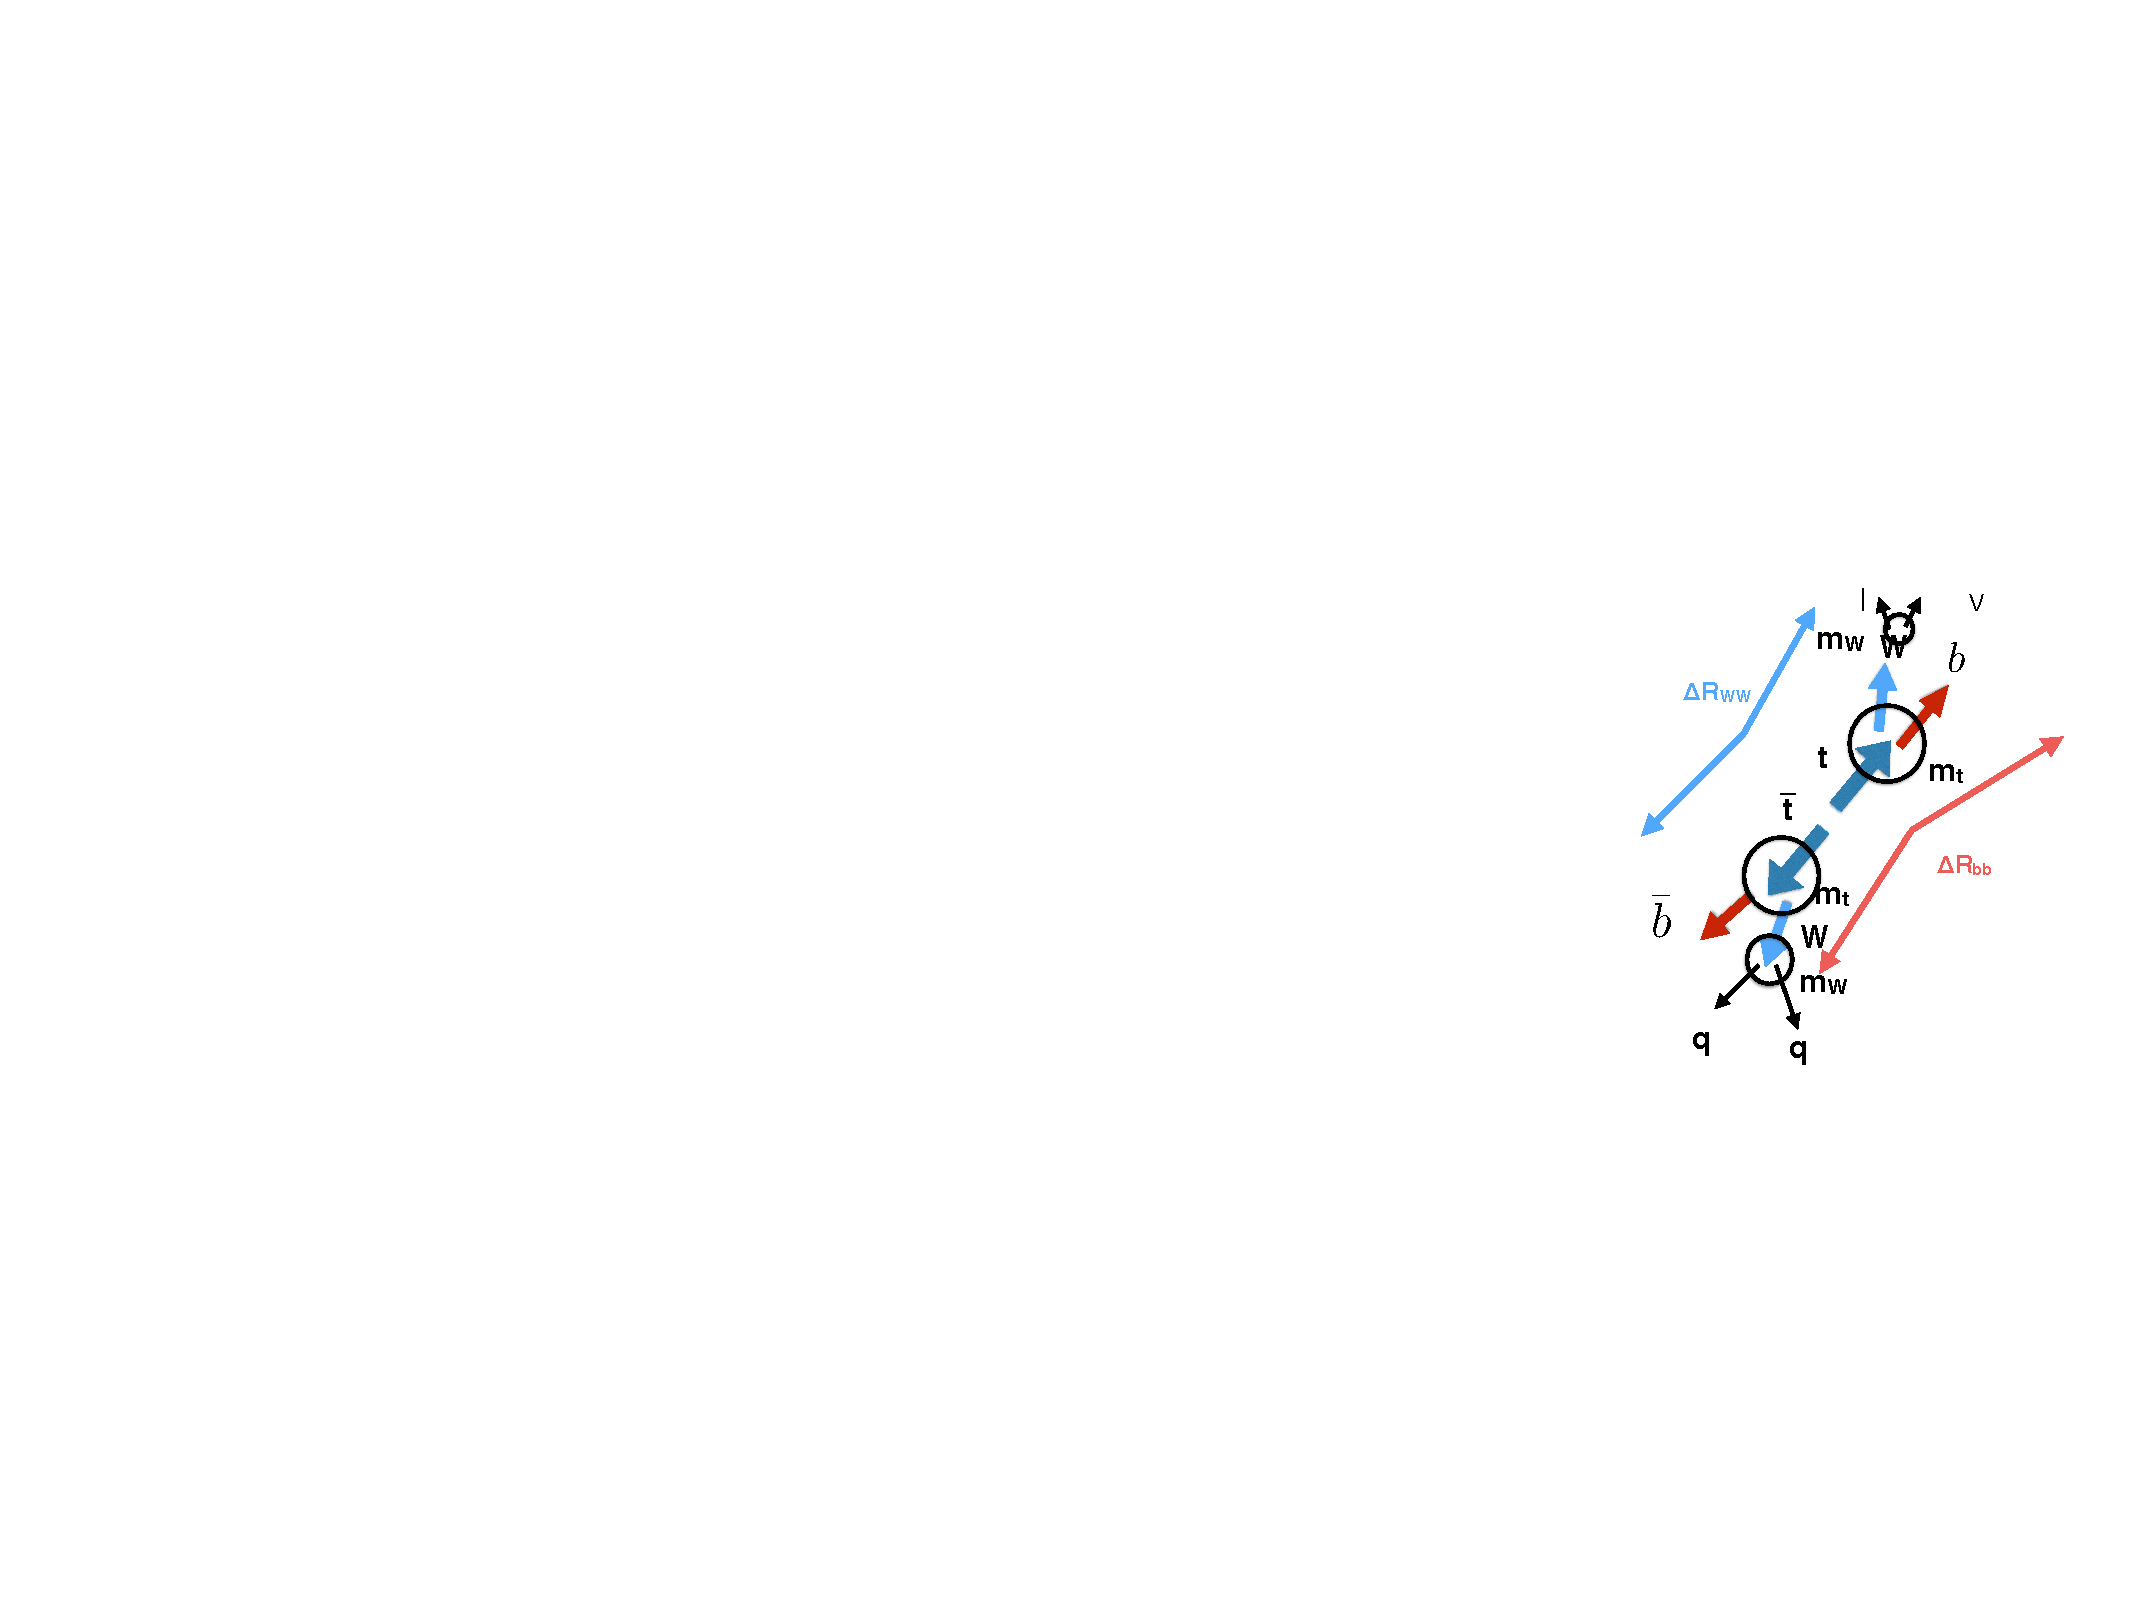
\includegraphics[width=0.45\textwidth]{figures/cartoon_tt}
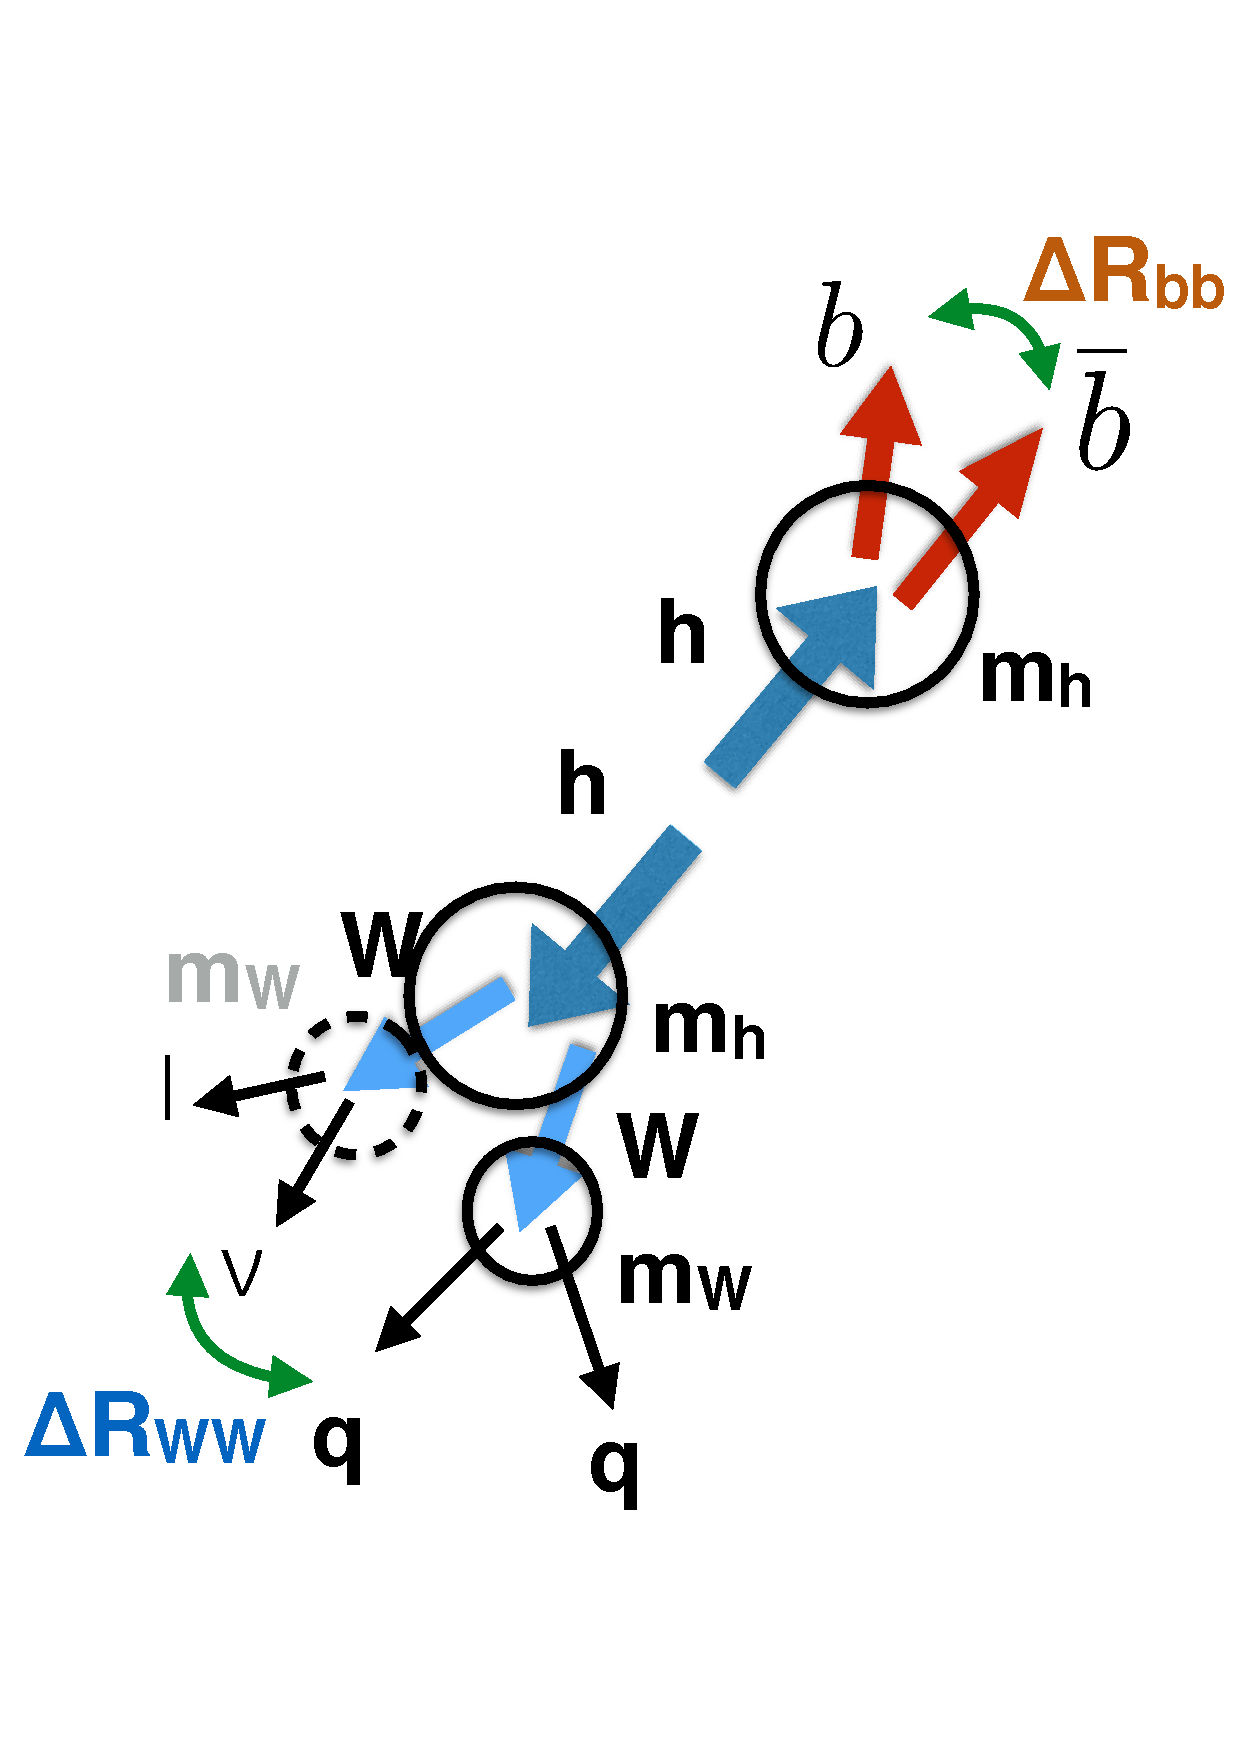
\includegraphics[width=0.45\textwidth]{figures/cartoon_hh_crop}
\end{center}
\end{column}
\end{columns}
\end{frame}

\begin{frame}
\begin{center}
\header{Resolved Event Selection}
\end{center}
\color{MyPurple}{Pre-selection}
\begin{itemize}
\item 1+ trigger matched electron or muon
\item 4+ jets, exactly 2 b-tags
\end{itemize}
\color{MyPurple}{Event Selection}\color{black}
\begin{columns}
\begin{column}{0.5\textwidth}
\begin{itemize}
\item $\met$
\item high $p_{T}^{WW}$ and $p_{T}^{bb}$
\item $m_{bb}\sim{}m_{H}$
\end{itemize}
\end{column}
\begin{column}{0.5\textwidth}
\begin{itemize}
\item $m_{HH}$ window
\begin{itemize}
\item Depends on resonant signal mass hypothesis
\item I helped develop an implement these windows 
\end{itemize}
\end{itemize}
\end{column}
\end{columns}
\end{frame}

\begin{frame}
\begin{center}
\header{Resolved Background Determination}
\end{center}
\begin{columns}
\begin{column}{0.5\textwidth}
\color{MyPurple}{\ttbar}
\begin{itemize}
\item Normalized in $m_{bb}$ CRs
\begin{itemize}
\item reversed $m_{bb}$ cut
\end{itemize}
\end{itemize}
\end{column}
\begin{column}{0.5\textwidth}
\color{MyPurple}{Other MC Bkg.}
\begin{itemize}
\item Modeled using MC and normilized to SM XSec
\end{itemize}
\end{column}
\end{columns}
\begin{center}
\color{MyPurple}{QCD multi-jet background}
\end{center}
\begin{columns}
\begin{column}{0.5\textwidth}
\begin{itemize}
\vspace{-0.5cm}
\item ABCD data driven estimate
\begin{itemize}
\item $N_A = F N_C N_B / N_D$
\item $F$ is a correction factor determined earlier in the cutflow
\item I developed the correction factor to overcome low stats in C region
\end{itemize}
\end{itemize}
\end{column}
\begin{column}{0.5\textwidth}
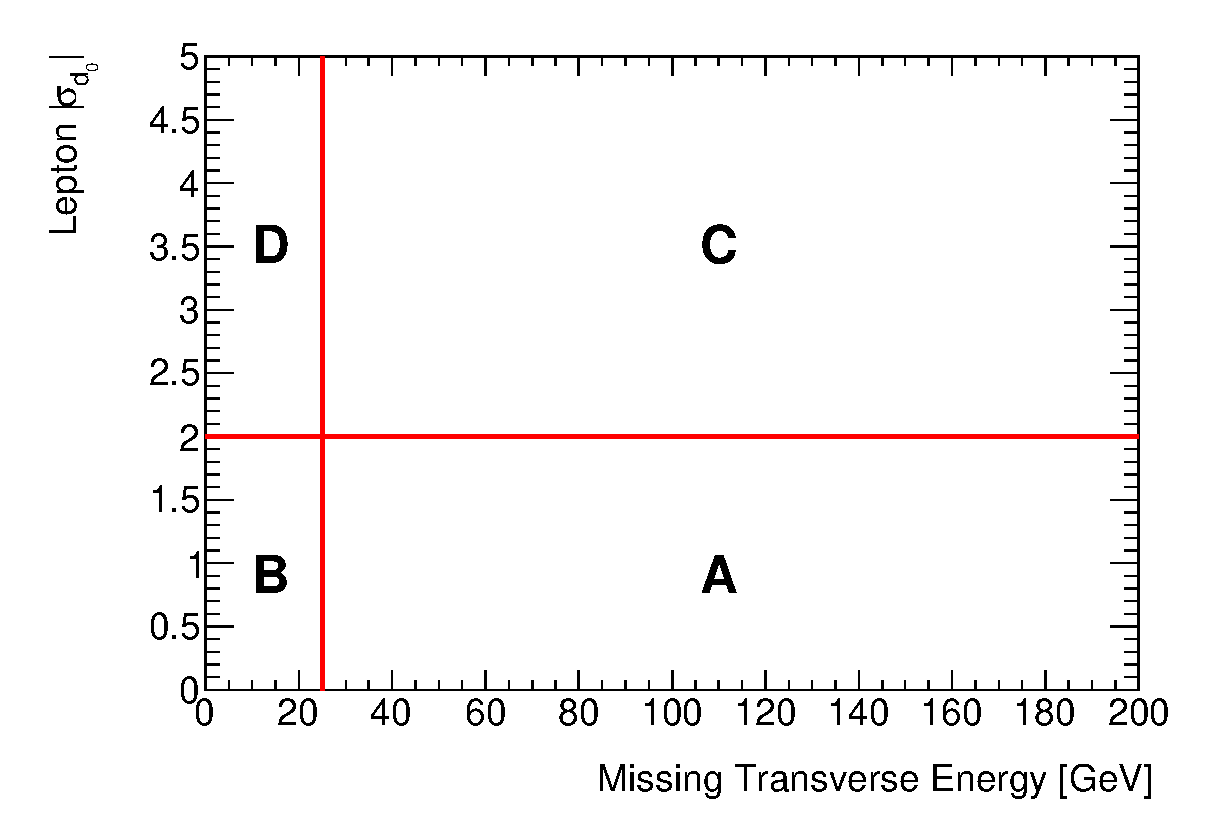
\includegraphics[width=0.9\textwidth]{figures/abcdExample_met_vs_d0sigBL20}
\end{column}
\end{columns}
\end{frame}

\begin{frame}
\begin{center}
\header{Resolved Background Shape Check}
\end{center}
\begin{center}
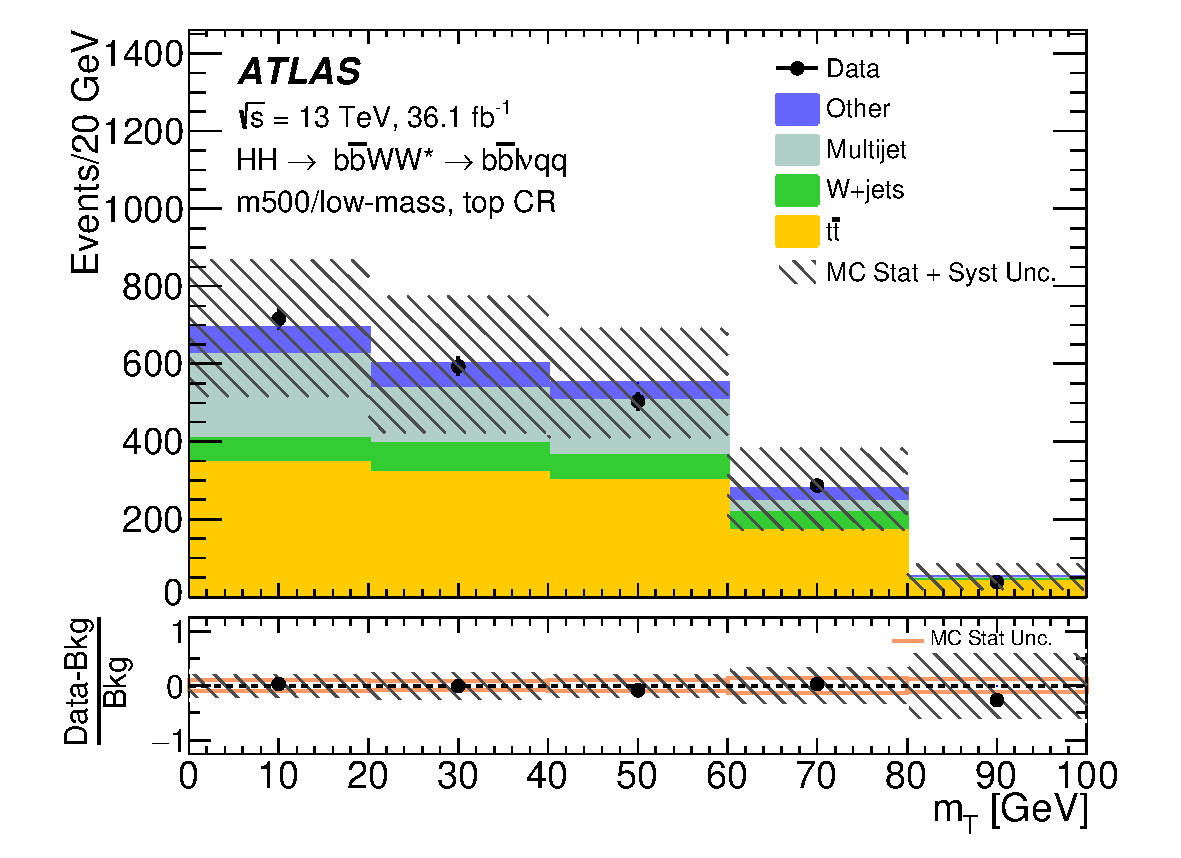
\includegraphics[width=0.8\textwidth]{figures/C_mBBcr_reOpt700_mww_bbpt210_wlepmtben_regionA_met25d020-eps-converted-to}
\end{center}
\small
$m_T = \sqrt{2p_T^l\met\times{}(1-\cos{\Delta{\phi}})}$
\end{frame}


\begin{frame}
\begin{center}
\header{Boosted Analysis}
\end{center}
\begin{columns}
\begin{column}{0.5\textwidth}
\color{MyPurple}{Signal Region}
\begin{itemize}
\footnotesize
\item slightly larger \met cut
\item $m_{\mathrm{Large-R}}\sim{}m_{H}$
\end{itemize}
\color{MyPurple}{Background Modeling}
\begin{itemize}
\footnotesize
\item \ttbar VR
\item Other MC Bkg: Normalized to SM XSec
\item Multijet: Similar to resolved
\begin{itemize}
\scriptsize
\item $\met > 50 \text{ GeV}$
\item $m_{HH}$ dist, taken from 1 b-tag selection
\end{itemize}
\end{itemize}
\end{column}
\begin{column}{0.5\textwidth}

\begin{center}
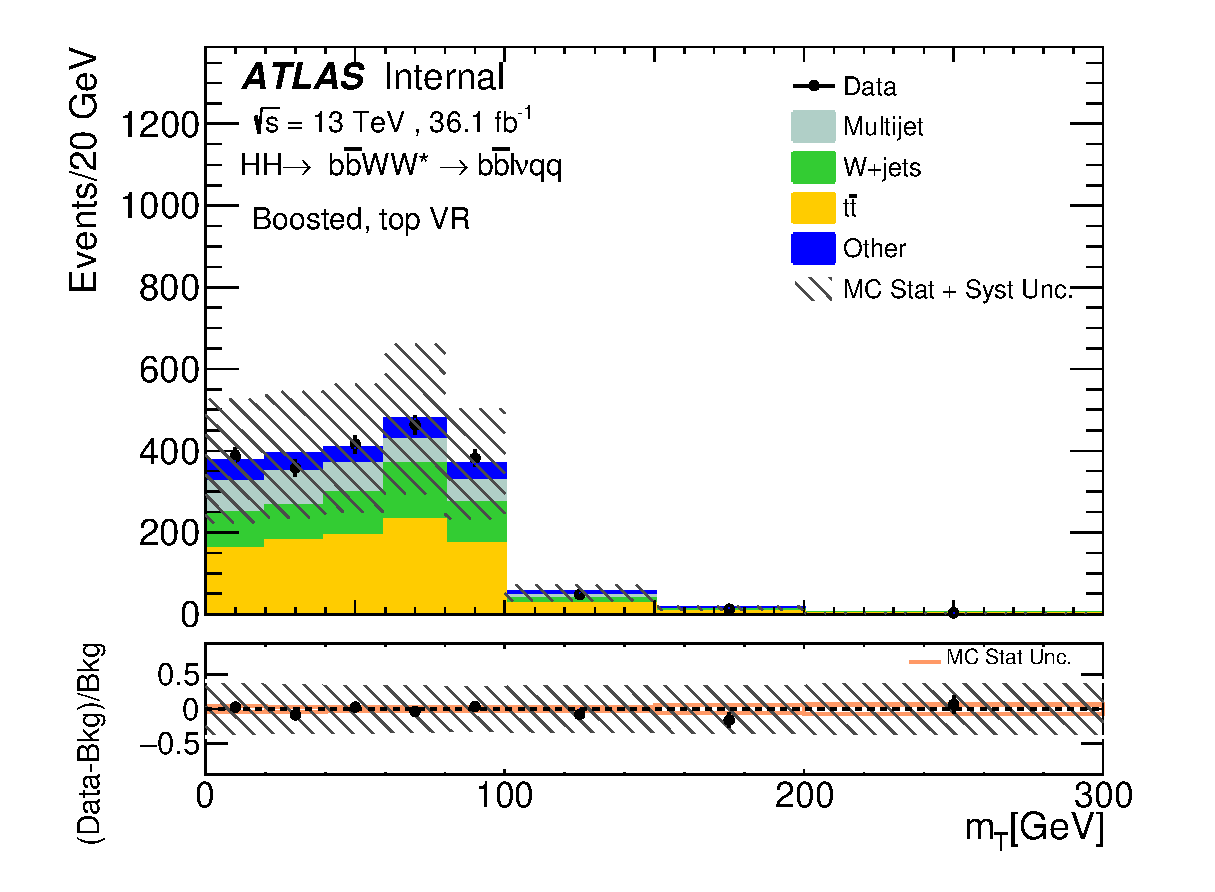
\includegraphics[width=1\textwidth]{figures/C_2tab_0bjet_mbbcr_lepton_presel_met50_WlepMtATLAS}
\end{center}
\end{column}
\end{columns}
\end{frame}

\begin{frame}
\begin{center}
\header{Results}
\end{center}
\begin{center}
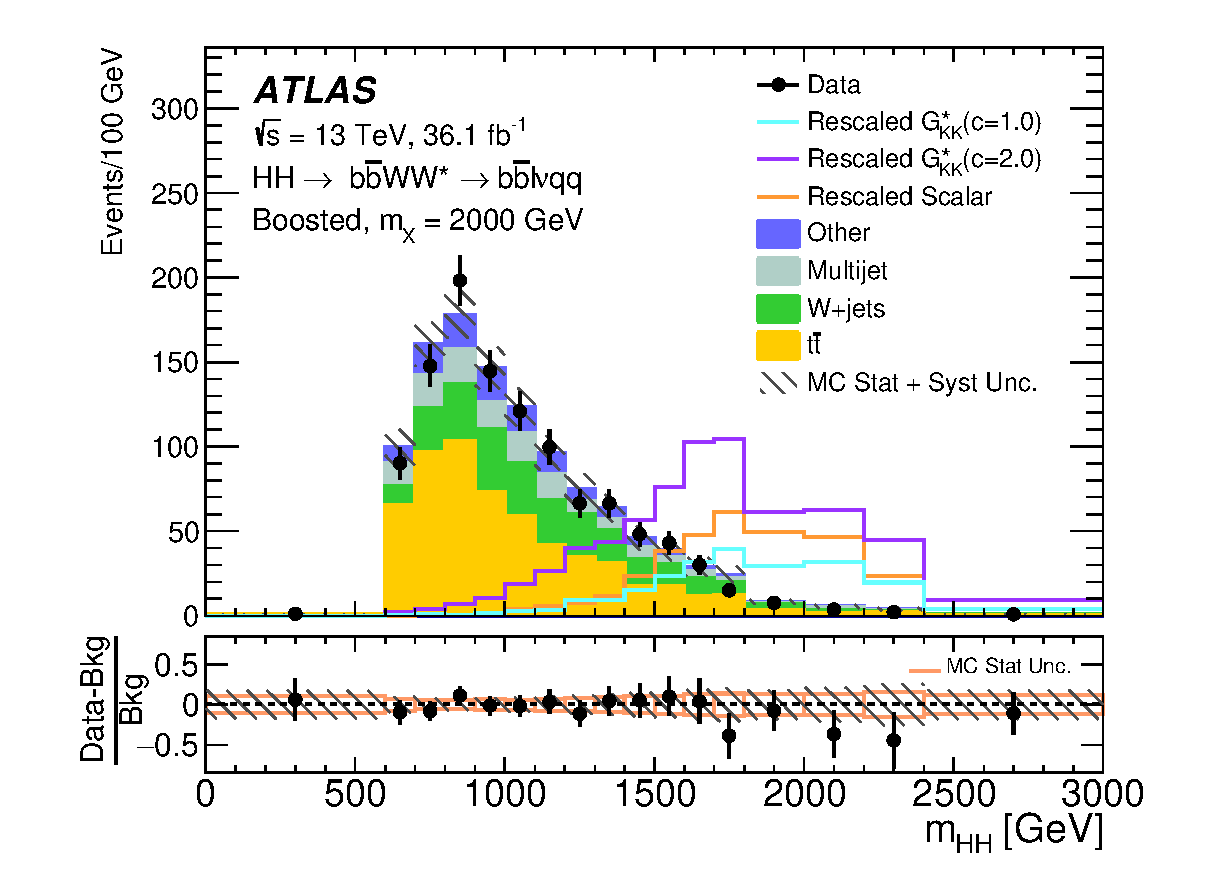
\includegraphics[width=0.8\textwidth]{figures/C_2tab_0bjet_SR_lepton_presel_met50_hhMassRebin1_postfit}
\end{center}
%\end{column}
%\end{columns}
\end{frame}

\begin{frame}
\begin{center}
\header{Combined Limit}
\end{center}
\begin{center}
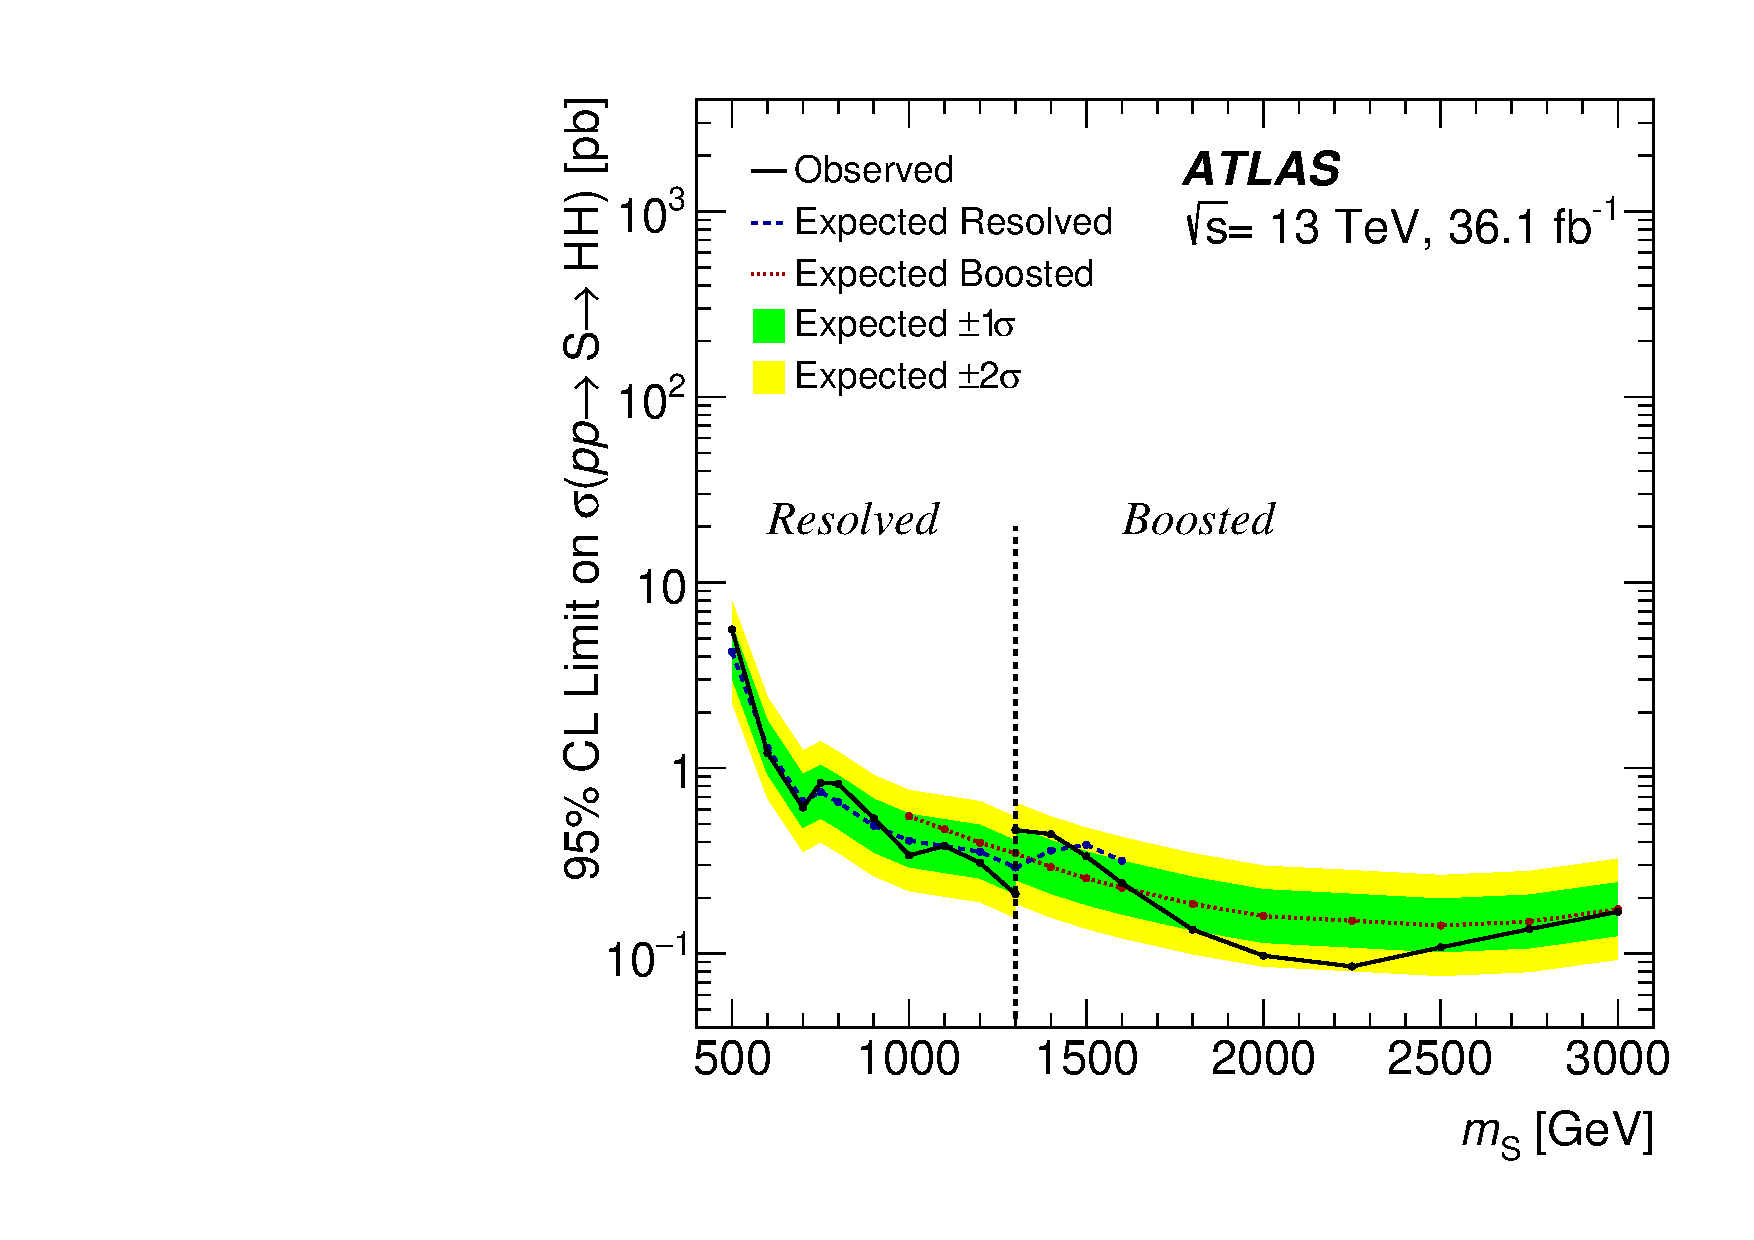
\includegraphics[width=0.7\textwidth]{figures/limit_2016_reOpt_HiggsApproved_Scalar_Paper_Combined_20190312_01}
\end{center}
\end{frame}

\begin{frame}
\begin{center}
\header{Improvements for Full Run II}
\end{center}
\vspace{-0.5cm}
\begin{columns}
\begin{column}{0.5\textwidth}
\color{MyPurple}{Motivation}
\begin{itemize}
\footnotesize
\item $H\rightarrow{}WW$ becomes boosted around 1 TeV 
\item Quarks become too close together to use 0.4 jets
\item Overlap removal with leptons kill efficiency
\item A "Fully-Boosted" selection recovers lost efficiency at high $m_S$
\end{itemize}
\end{column}
\begin{column}{0.5\textwidth}
\begin{center}
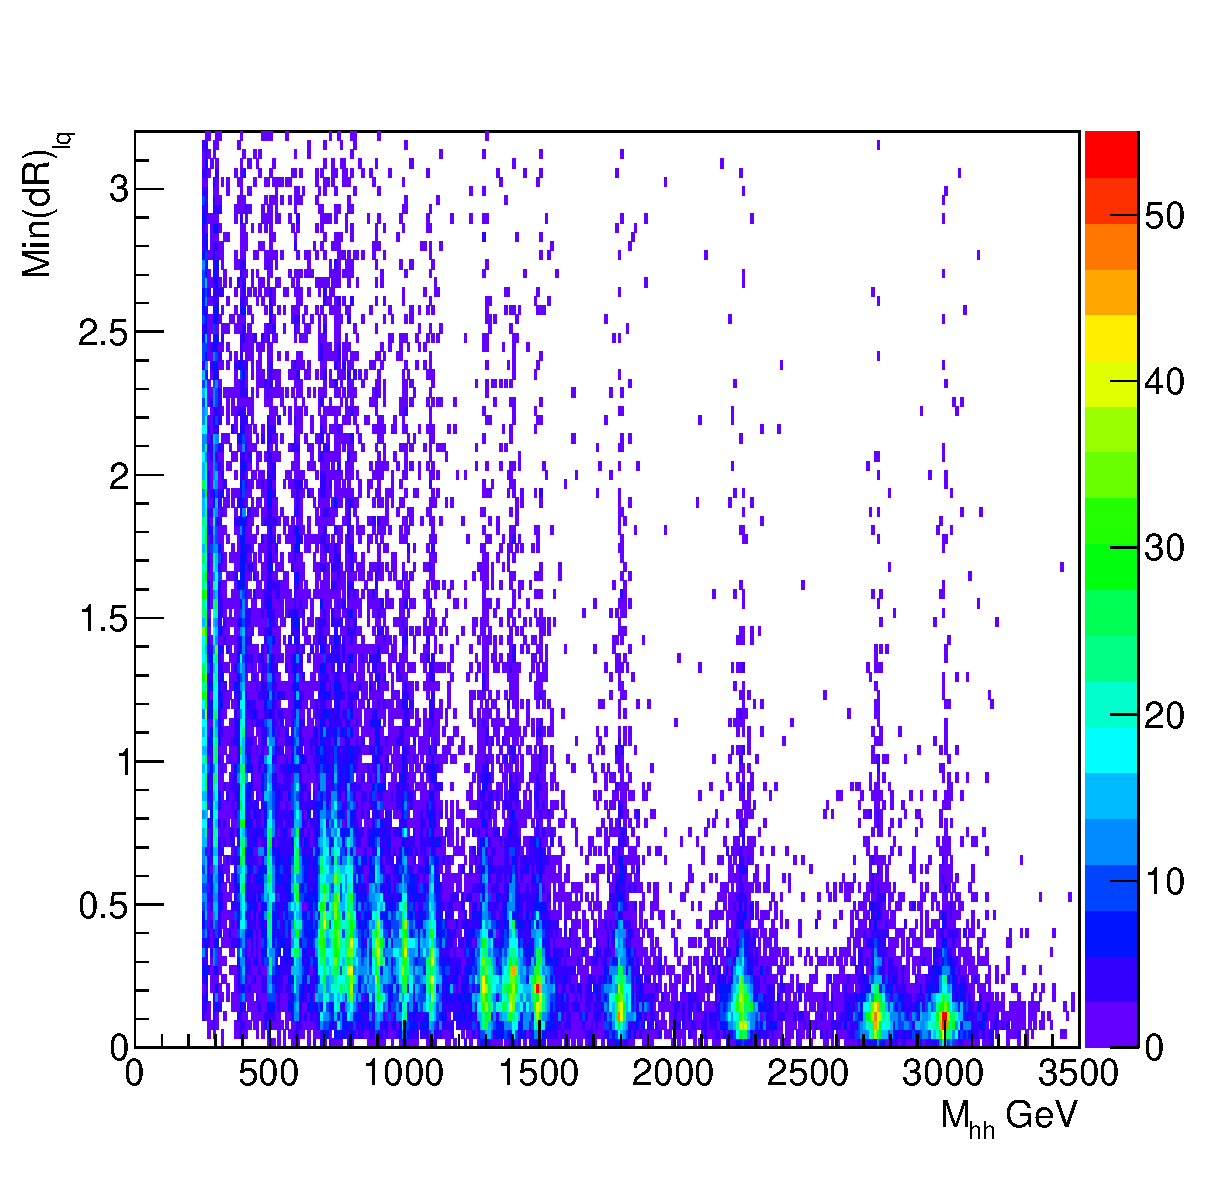
\includegraphics[width=0.75\textwidth]{figures/drminlq}
\end{center}
\end{column}
\end{columns}
\end{frame}

\begin{frame}
\begin{center}
\header{Event Selection}
\end{center}
\begin{center}
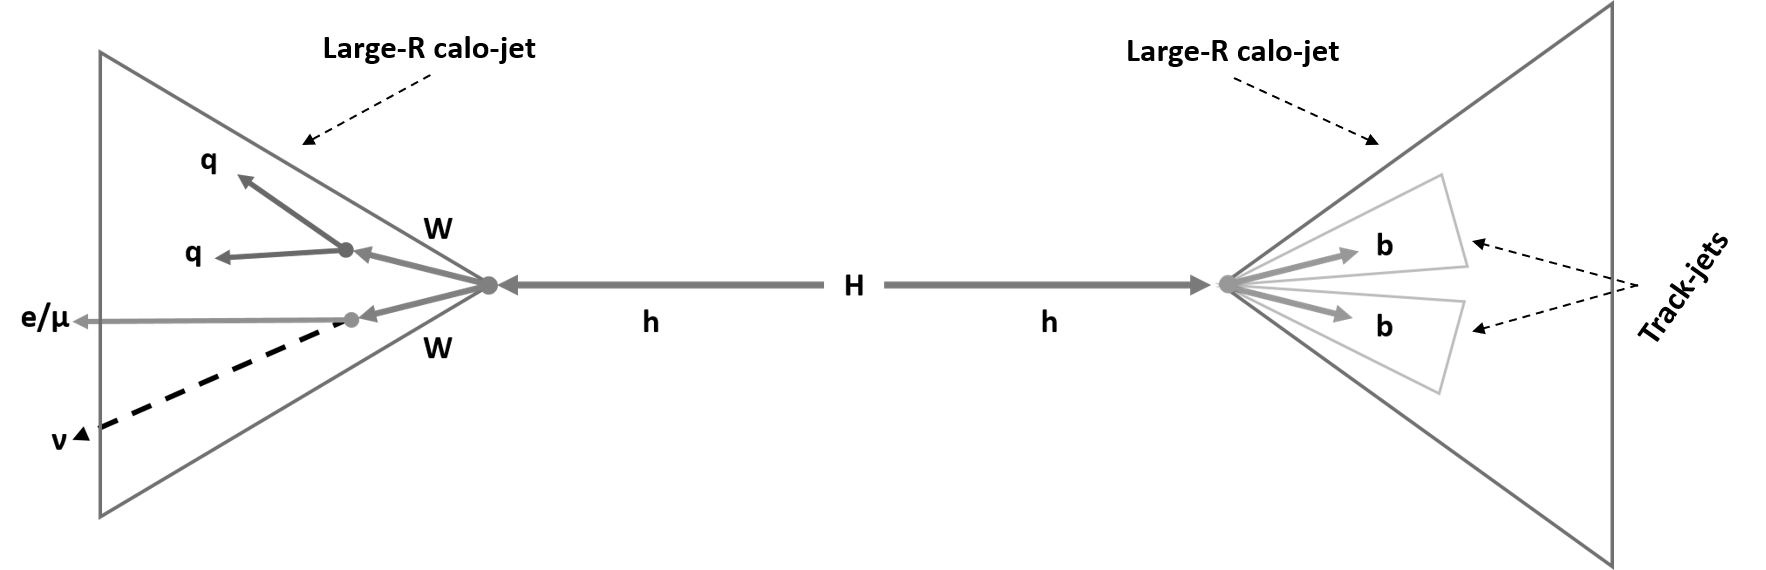
\includegraphics[width=0.9\textwidth]{figures/full_boosted}
\end{center}
\end{frame}

\begin{frame}
\begin{center}
\header{Signal Reconstruction}
\end{center}
\begin{columns}
\begin{column}{0.5\textwidth}
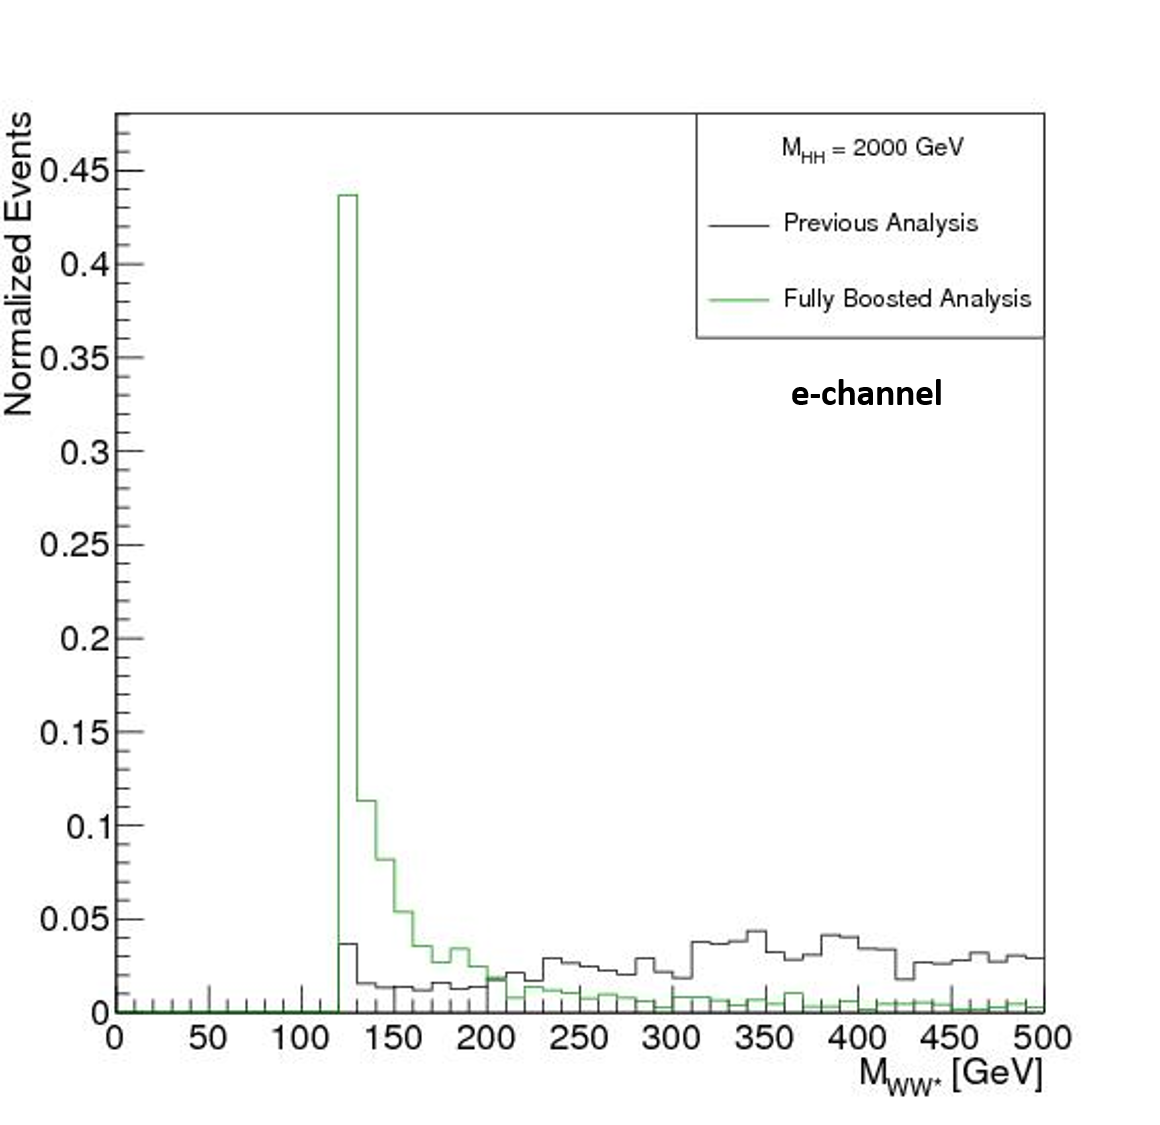
\includegraphics[width=01\textwidth]{figures/electron/mww_e}
\end{column}
\begin{column}{0.5\textwidth}
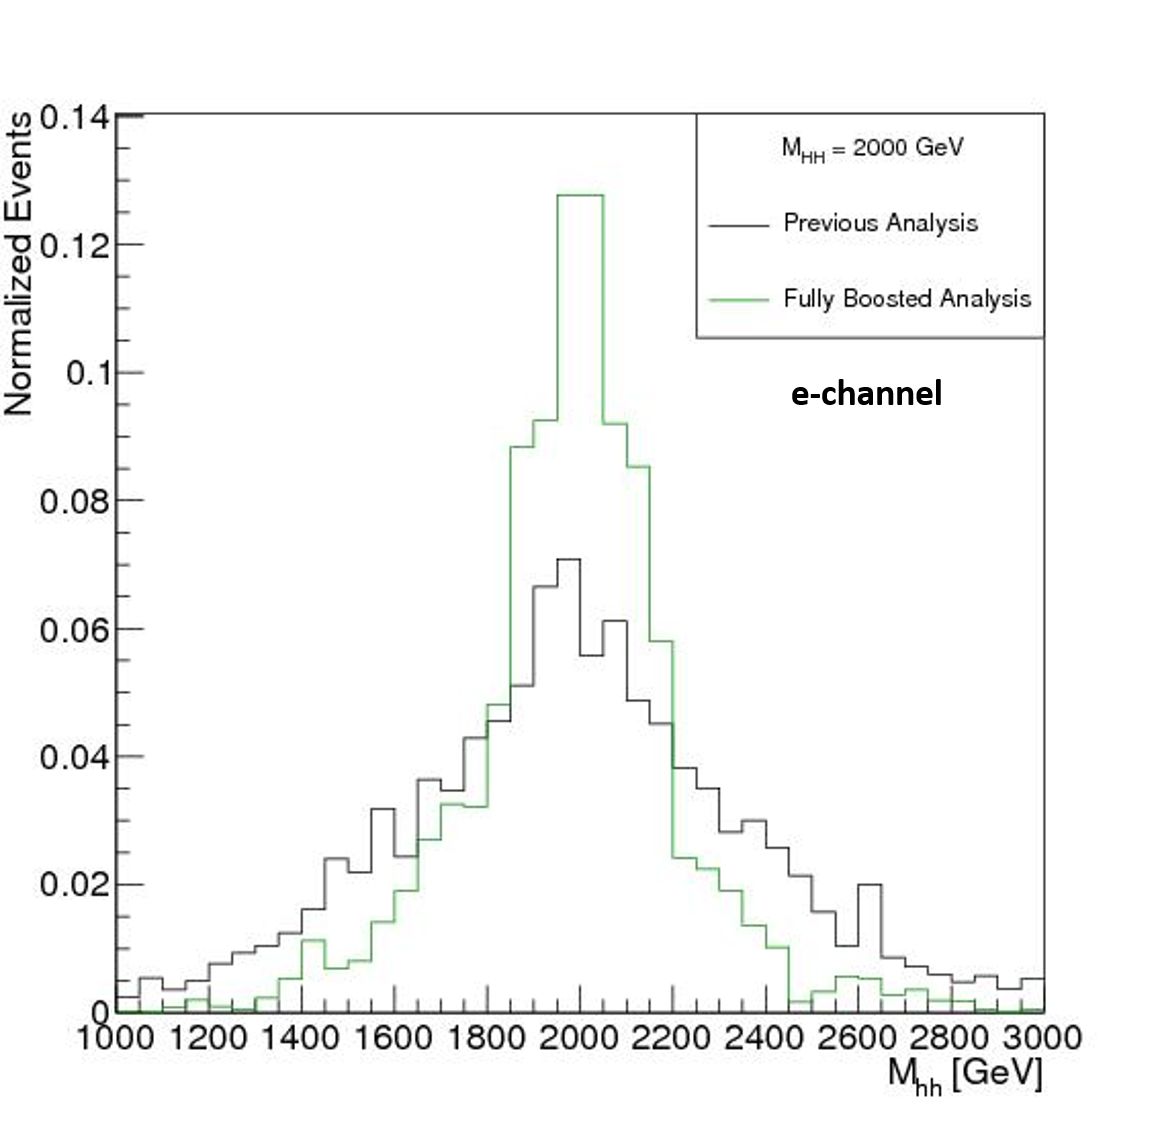
\includegraphics[width=01\textwidth]{figures/electron/mhh_e}
\end{column}
\end{columns}
%\begin{columns}
%\begin{column}{0.3\textwidth}
%\small
%\color{MyPurple}{$H\rightarrow{}b\bar{b}$}
%\begin{itemize}
%\footnotesize
%\item Same as boosted analysis
%\end{itemize}
%\small
%\color{MyPurple}{$H\rightarrow{}WW^{*}$}
%\begin{itemize}
%\footnotesize
%\item ID trigger lepton
%\item Large-R jet:
%\begin{itemize}
%\scriptsize
%\item $e$ channel: Jet
%\item $\mu$ channel: Jet + $\mu$
%\end{itemize}
%\item Reconstructed $\nu$
%\end{itemize}
%\end{column}
%\begin{column}{0.7\textwidth}
%\begin{center}
%\vspace{-0.5cm}
%\hspace{-0.5cm}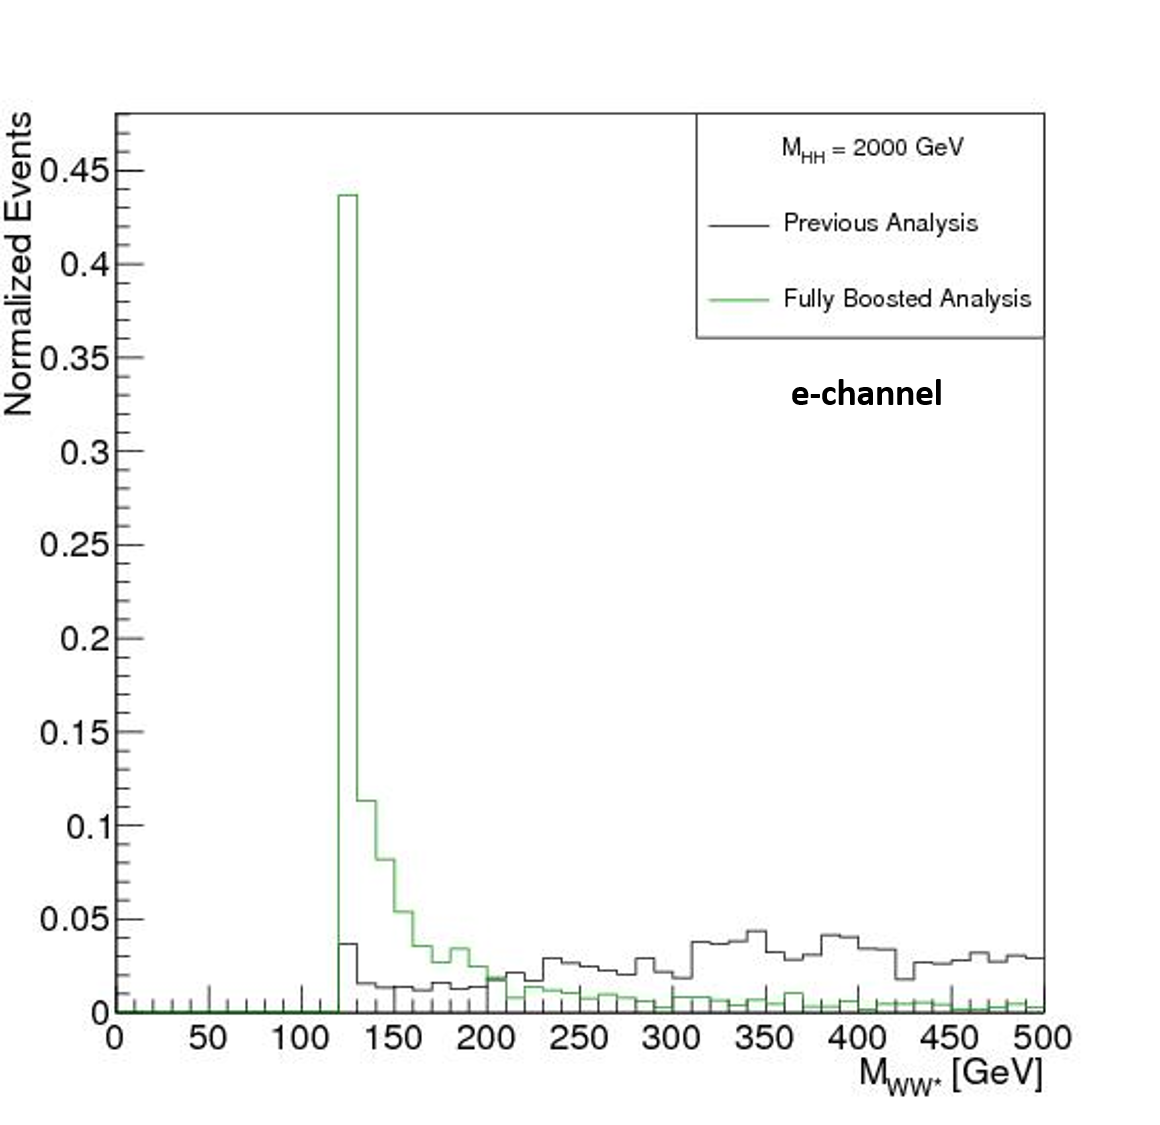
\includegraphics[width=0.5\textwidth]{figures/electron/mww_e}\\
%\hspace{-0.5cm}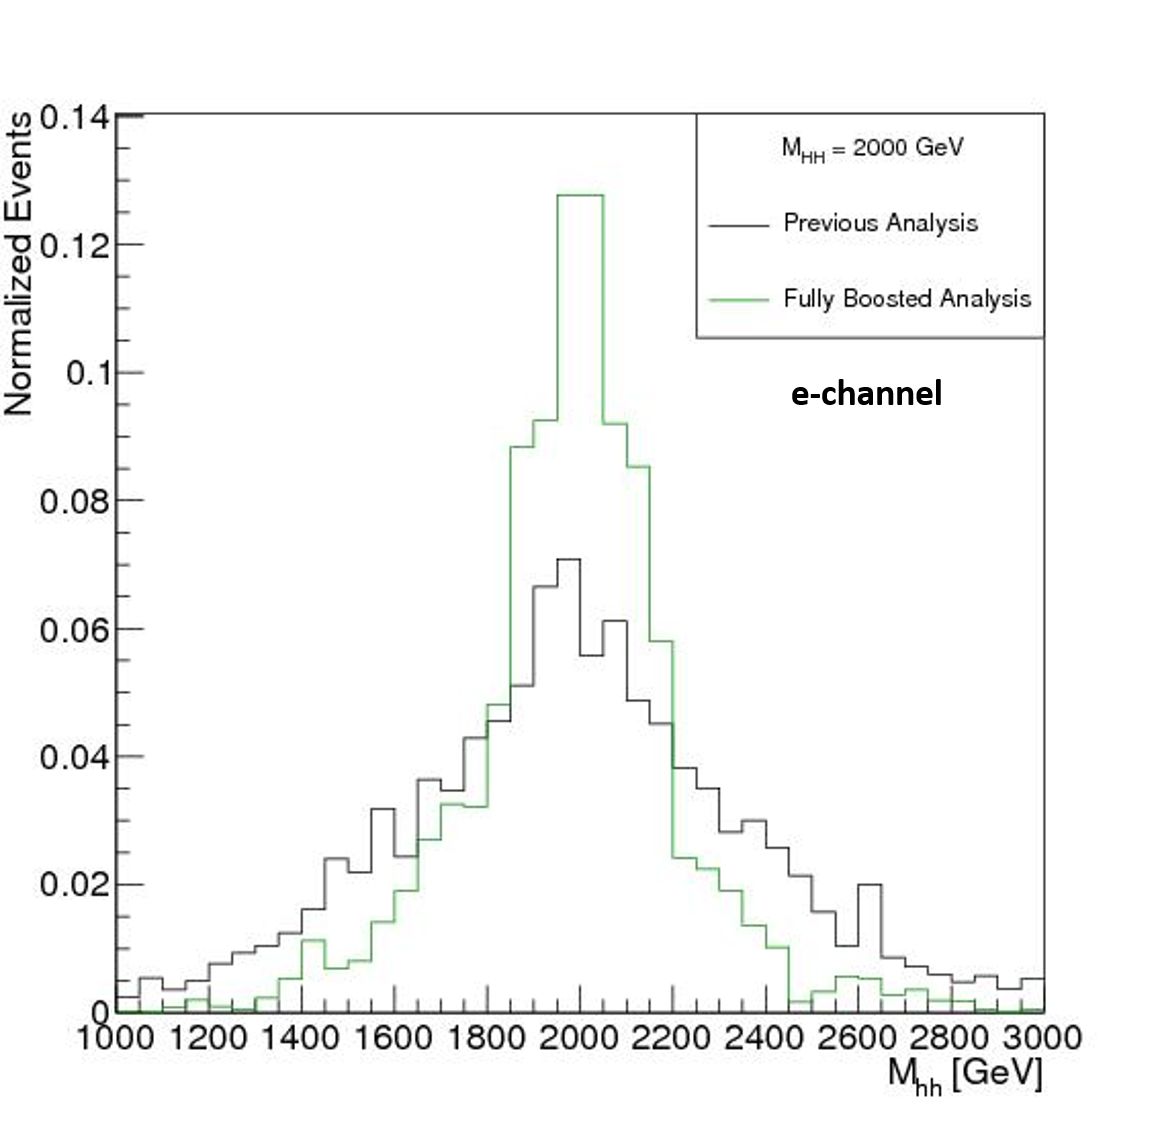
\includegraphics[width=0.5\textwidth]{figures/electron/mhh_e}
%\end{center}
%\end{column}
%\end{columns}
\end{frame}

\begin{frame}
\begin{center}
\header{Background Modeling}
\end{center}
{\color{MyPurple}{Similar to Boosted Analysis}}
\begin{columns}
\begin{column}{0.5\textwidth}
\vspace{-1cm}
\begin{itemize}
\item \ttbar checked in $m_{bb}$ VR
\item QCD multijet: ABCD method
\item Other: Norm to SM XSec
\end{itemize}
\end{column}
\begin{column}{0.5\textwidth}
\vspace{-0.9cm}
\begin{table}
\begin{center}
\scriptsize
\begin{tabular}{|l|c|c|c}
\hline
Sample        &  Yield   &  Stats Unc \\ 
\hline 
$t\bar{t}$    &  187.7  & $\pm$ 8.8    \\
W+Jets        &  33.7   & $\pm$ 1.9     \\
QCD           &  34.5   & $\pm$ 5.5     \\
Single-top    &  7.0   & $\pm$ 1.3     \\
Z+Jets        &  4.7    & $\pm$ 0.4        \\
Dibosons      &  3.3    & $\pm$ 0.6      \\
\hline
Prediction    &  271.0  & $\pm$ 10.7       \\
Data          &  268    & - \\
\hline
Data/Pred     &  0.99    & -  \\
\hline
\end{tabular}
\end{center}
\end{table}
\end{column}
\end{columns}
\begin{center}
\vspace{-0.4cm}
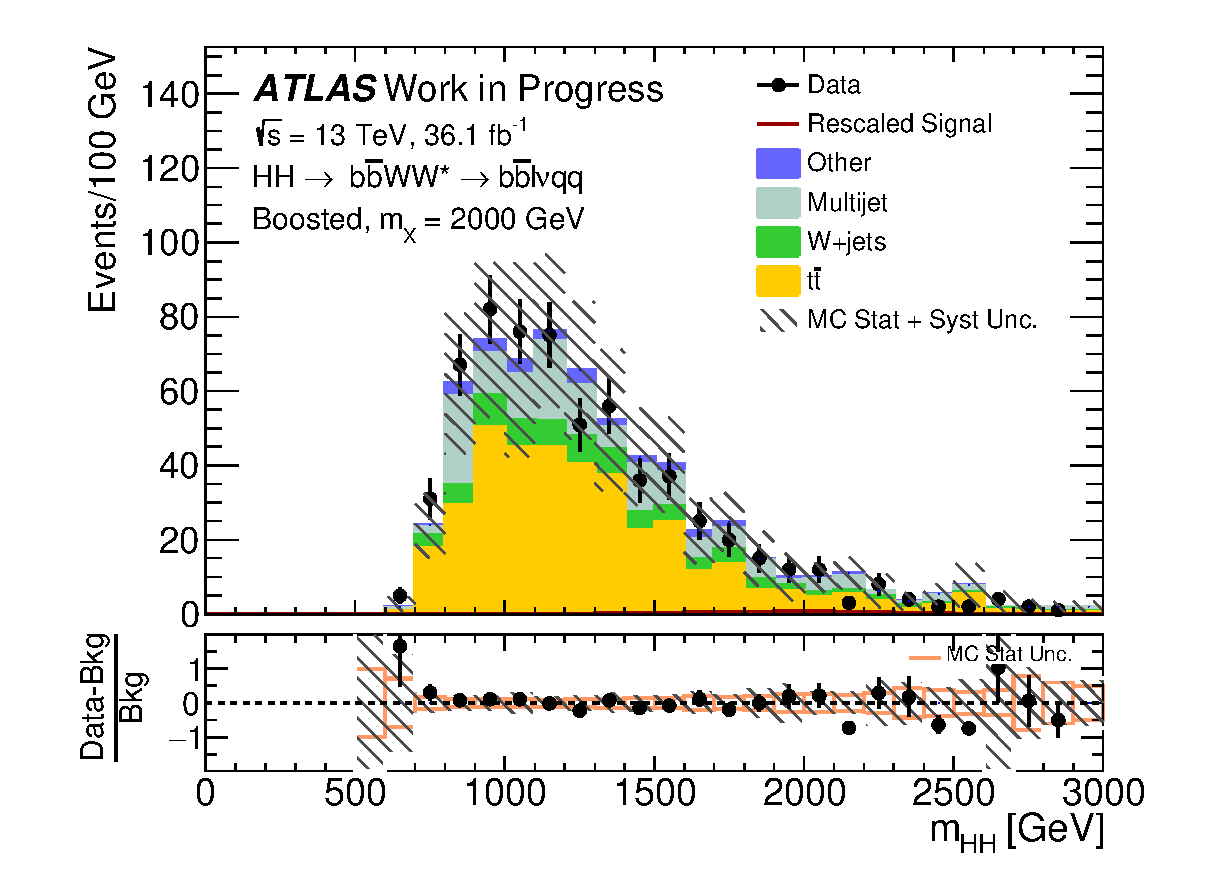
\includegraphics[width=0.5\textwidth]{figures/C_2tag_mbbcr_lepton_presel_met50_hhMassRebin1}
\end{center}
\end{frame}

\begin{frame}
\begin{center}
\header{Results}
\end{center}
\vspace{-0.2cm}
\begin{center}
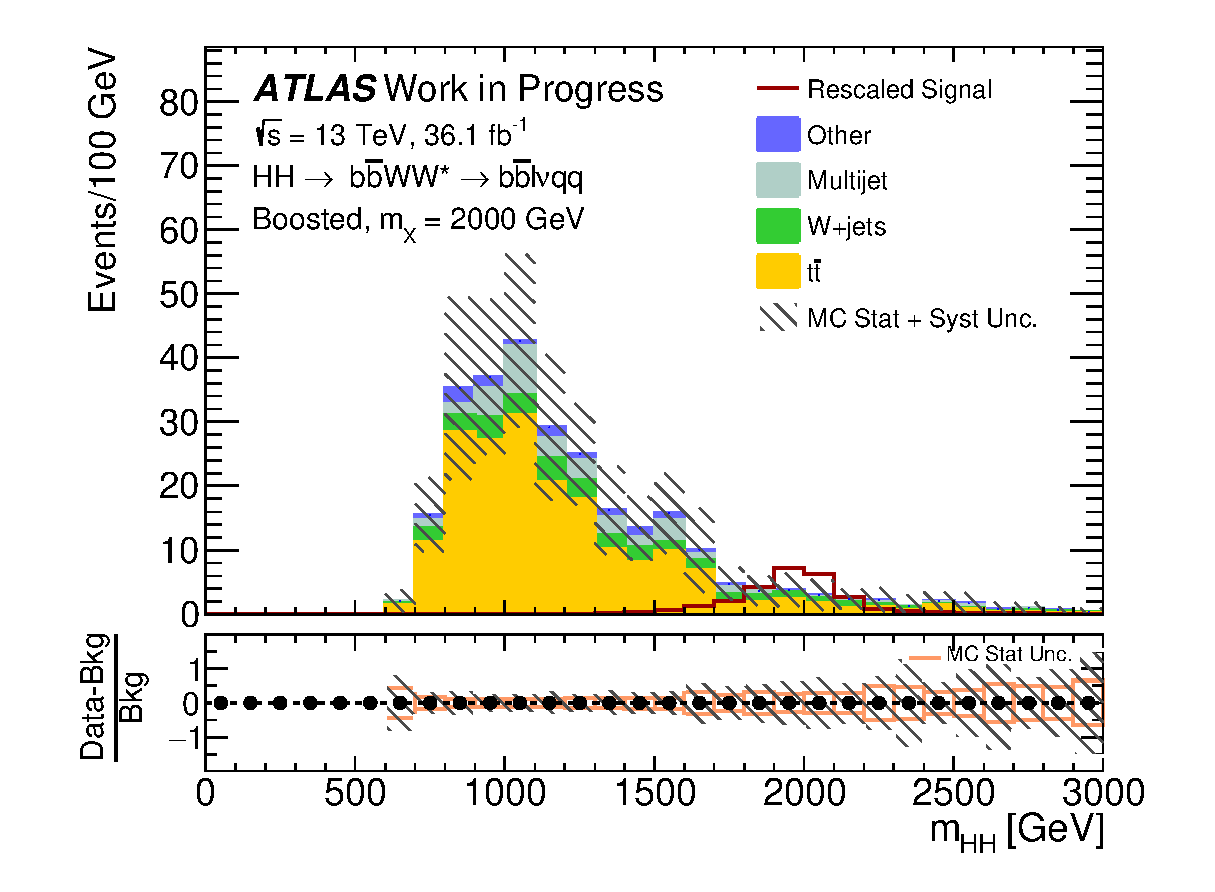
\includegraphics[width=0.9\textwidth]{figures/C_2tag_SR_lepton_presel_met50_hhMassRebin1}
\end{center}
\end{frame}

\begin{frame}
\begin{center}
\header{Results}
\end{center}
\begin{columns}
\begin{column}{0.5\textwidth}
\begin{center}
\color{MyPurple}{Published Analysis}
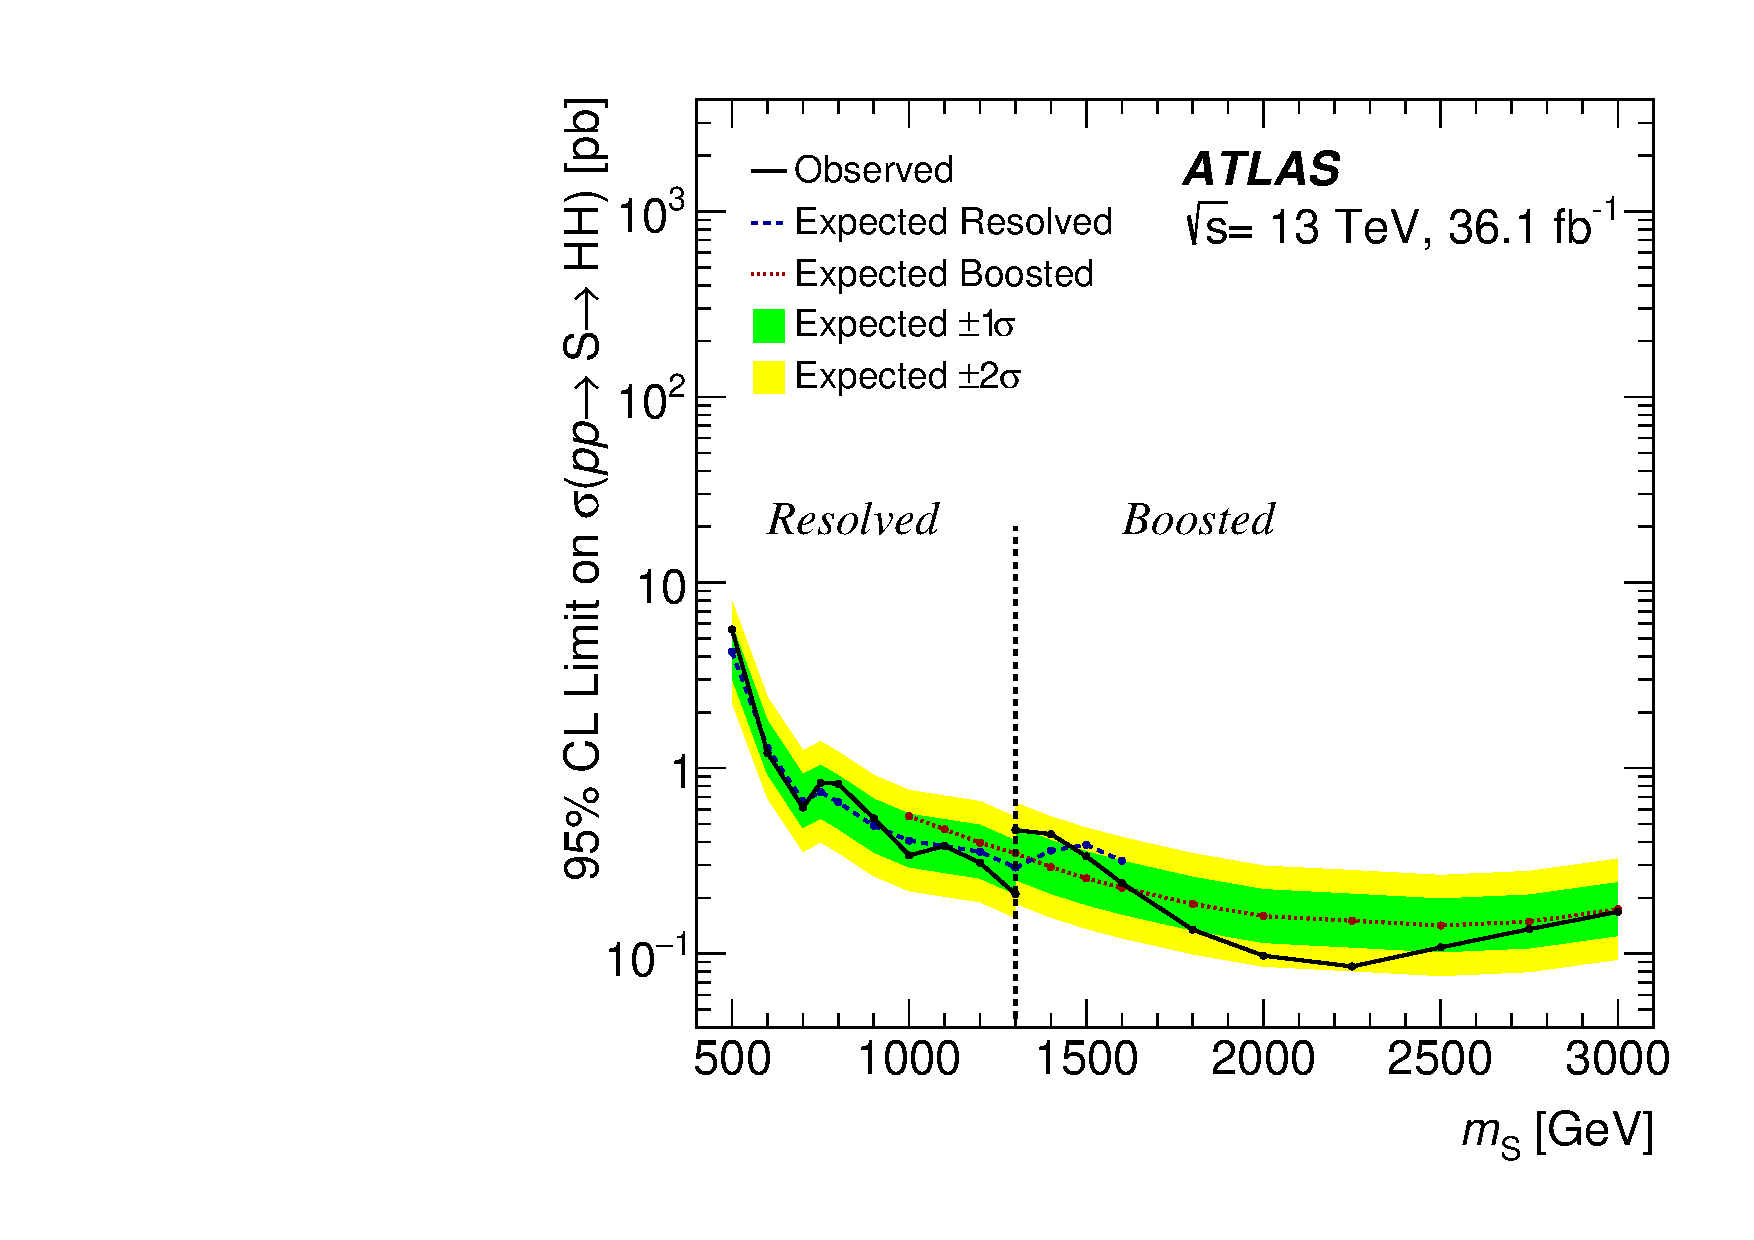
\includegraphics[width=01\textwidth]{figures/limit_2016_reOpt_HiggsApproved_Scalar_Paper_Combined_20190312_01}
\end{center}
\end{column}
\begin{column}{0.5\textwidth}
\begin{center}
\color{MyPurple}{Improved Analysis}
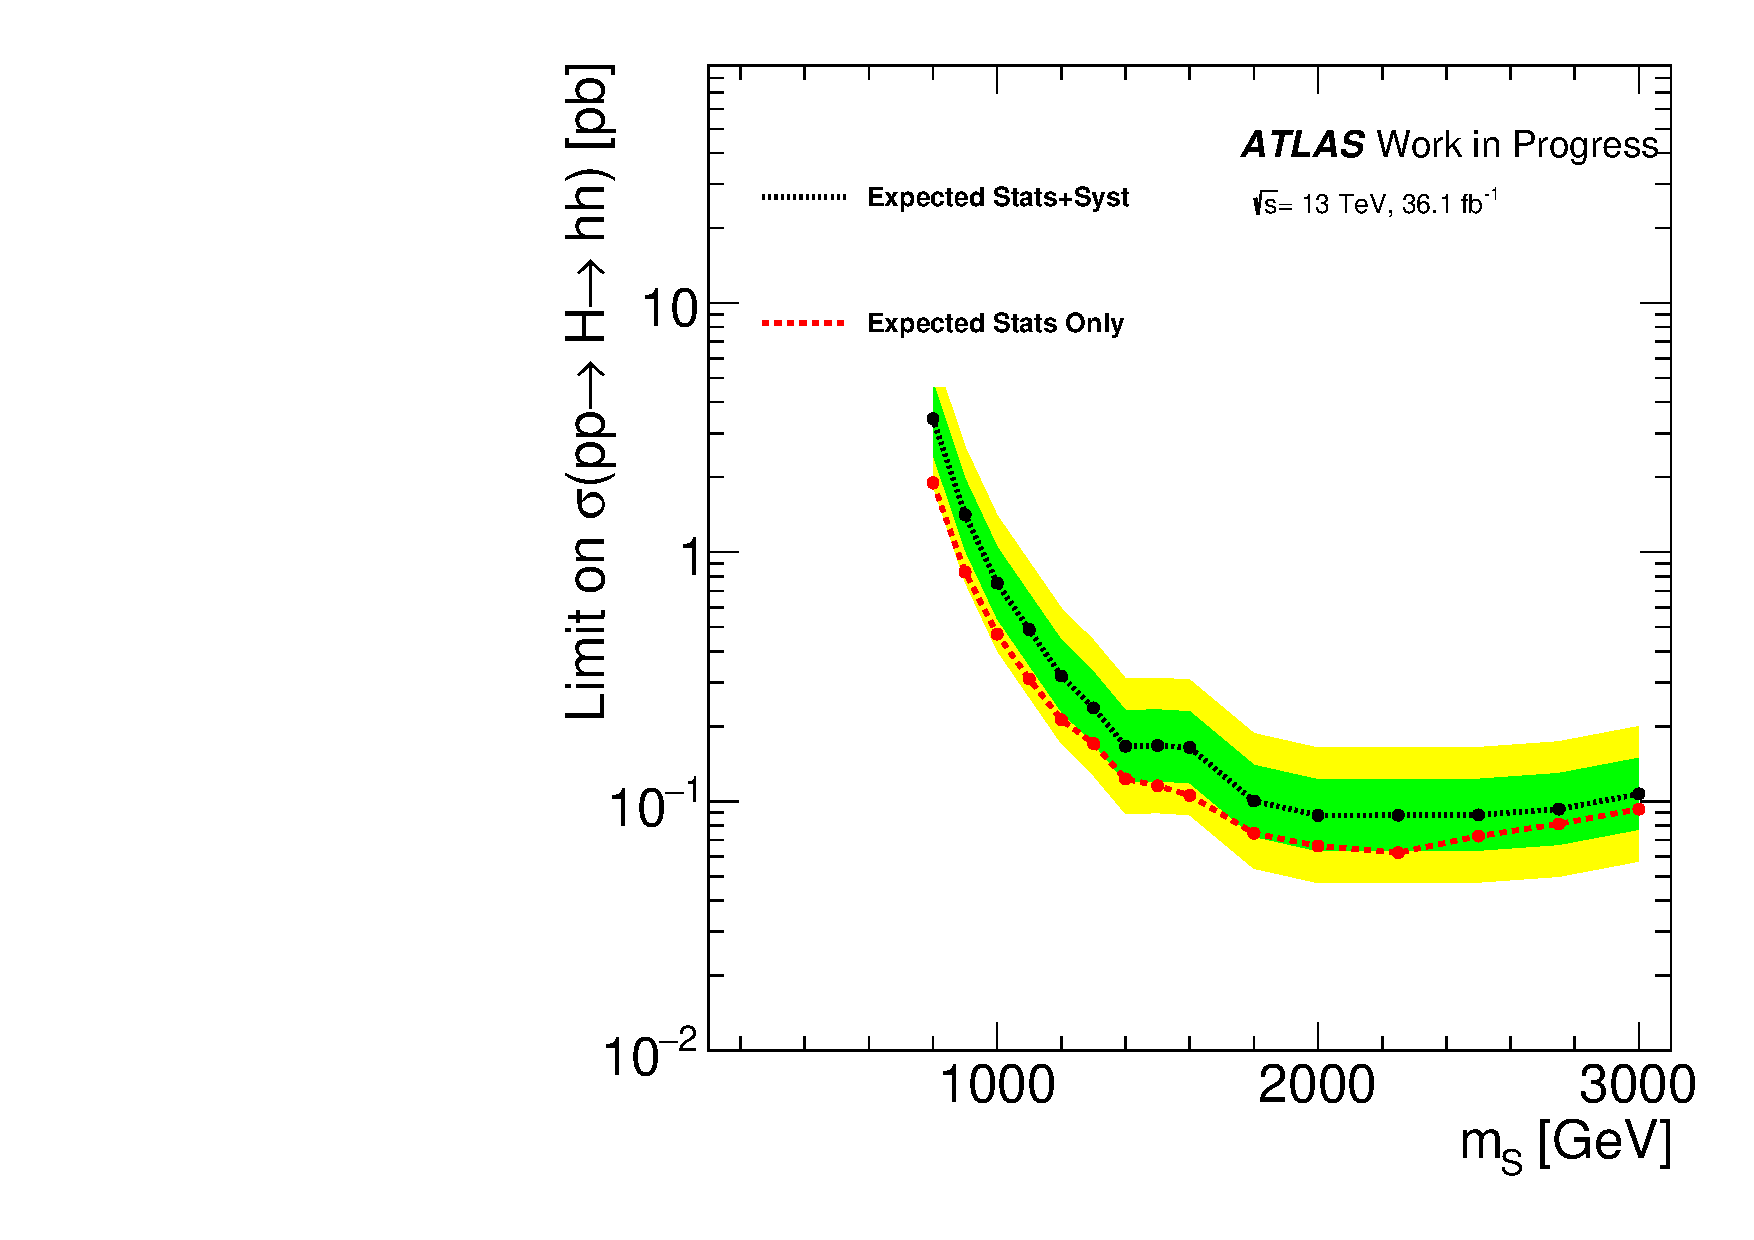
\includegraphics[width=01\textwidth]{figures/Final_limits}
\end{center}
\end{column}
\end{columns}
\end{frame}



\appendix
\backupbegin
\begin{frame}
\begin{center}
\fontsize{16}{8}\selectfont \textbf{{\color{MyPurple}{Backup}}}\\~\\
\end{center}
\end{frame}


\backupend
\end{document}


